%% abtex2-modelo-trabalho-academico.tex, v-1.9.2 laurocesar
%% Copyright 2012-2014 by abnTeX2 group at http://abntex2.googlecode.com/ 
%%
%% This work may be distributed and/or modified under the
%% conditions of the LaTeX Project Public License, either version 1.3
%% of this license or (at your option) any later version.
%% The latest version of this license is in
%%   http://www.latex-project.org/lppl.txt
%% and version 1.3 or later is part of all distributions of LaTeX
%% version 2005/12/01 or later.
%%
%% This work has the LPPL maintenance status `maintained'.
%% 
%% The Current Maintainer of this work is the abnTeX2 team, led
%% by Lauro César Araujo. Further information are available on 
%% http://abntex2.googlecode.com/
%%
%% This work consists of the files abntex2-modelo-trabalho-academico.tex,
%% abntex2-modelo-include-comandos and abntex2-modelo-references.bib
%%

% ------------------------------------------------------------------------
% ------------------------------------------------------------------------
% abnTeX2: Modelo de Trabalho Academico (tese de doutorado, dissertacao de
% mestrado e trabalhos monograficos em geral) em conformidade com 
% ABNT NBR 14724:2011: Informacao e documentacao - Trabalhos academicos -
% Apresentacao
% ------------------------------------------------------------------------
% ------------------------------------------------------------------------

\documentclass[
	% -- opções da classe memoir --
	12pt,				% tamanho da fonte
	openright,			% capítulos começam em pág ímpar (insere página vazia caso preciso)
	twoside,			% para impressão em verso e anverso. Oposto a oneside
	a4paper,			% tamanho do papel. 
	% -- opções da classe abntex2 --
	%chapter=TITLE,		% títulos de capítulos convertidos em letras maiúsculas
	%section=TITLE,		% títulos de seções convertidos em letras maiúsculas
	%subsection=TITLE,	% títulos de subseções convertidos em letras maiúsculas
	%subsubsection=TITLE,% títulos de subsubseções convertidos em letras maiúsculas
	% -- opções do pacote babel --
	english,			% idioma adicional para hifenização
	french,				% idioma adicional para hifenização
	spanish,			% idioma adicional para hifenização
	brazil				% o último idioma é o principal do documento
	]{abntex2}

% ---
% Pacotes básicos 
% ---
\usepackage{lmodern}			% Usa a fonte Latin Modern			
\usepackage[T1]{fontenc}		% Selecao de codigos de fonte.
\usepackage[utf8]{inputenc}		% Codificacao do documento (conversão automática dos acentos)
\usepackage{lastpage}			% Usado pela Ficha catalográfica
\usepackage{indentfirst}		% Indenta o primeiro parágrafo de cada seção.
\usepackage{color}				% Controle das cores
\usepackage{graphicx}			% Inclusão de gráficos
\usepackage{microtype} 			% para melhorias de justificação
\usepackage[final]{pdfpages}
\usepackage{url}
\usepackage{float}
\usepackage{amsmath}
\usepackage{cleveref}
\usepackage{pgfplots}
\usepackage{amsfonts}
\usepackage{amsmath}
\usepackage{tikz}
\usetikzlibrary{matrix, positioning}
\usepackage{tabularx}
\usepackage{mathtools}
\DeclareMathOperator{\logsumexp}{logsumexp}
\pgfmathdeclarefunction{sumexp}{3}{%
  \begingroup%
  \pgfkeys{/pgf/fpu}% "/pgf/fpu/output format=fixed" removed
  \pgfmathsetmacro{\myx}{#1}%
  \pgfmathtruncatemacro{\myxmin}{#2}%
  \pgfmathtruncatemacro{\myxmax}{#3}%
  \pgfmathsetmacro{\mysum}{0}%
  \pgfplotsforeachungrouped\XX in {\myxmin,...,\myxmax}%
    {\pgfmathsetmacro{\mysum}{\mysum+exp(\XX)}}%
  \pgfmathparse{\mysum+exp(#1)}%
  \pgfmathfloattofixed\pgfmathresult%  added
  \pgfmathsmuggle\pgfmathresult\endgroup%
}


\crefname{figure}{Figura}{Figuras}
\crefname{equation}{Equação}{Equações}
% ---
		
% ---
% Pacotes adicionais, usados apenas no âmbito do Modelo Canônico do abnteX2
% ---
\usepackage{lipsum}				% para geração de dummy text
% ---

% ---
% Pacotes de citações
% ---
\usepackage[brazilian,hyperpageref]{backref}	 % Paginas com as citações na bibl
\usepackage[alf]{abntex2cite}	% Citações padrão ABNT

% --- 
% CONFIGURAÇÕES DE PACOTES
% --- 

% ---
% Configurações do pacote backref
% Usado sem a opção hyperpageref de backref
\renewcommand{\backrefpagesname}{Citado na(s) página(s):~}
% Texto padrão antes do número das páginas
\renewcommand{\backref}{}
% Define os textos da citação
\renewcommand*{\backrefalt}[4]{
	\ifcase #1 %
		Nenhuma citação no texto.%
	\or
		Citado na página #2.%
	\else
		Citado #1 vezes nas páginas #2.%
	\fi}%
% ---

% ---
% Informações de dados para CAPA e FOLHA DE ROSTO
% ---
\titulo{Geração procedural de mapas de ilhas 2d com biomas através de técnicas de segmentação de imagem}
\autor{Lucas da Silva dos Santos\\Matheus Zanivan Andrade\\ Rafael Nascimento Lourenço}
\local{São Paulo - Brasil}
\data{2023}
\orientador{Lauro César Araujo}
\coorientador{Equipe \abnTeX}
\instituicao{%
  Senac: Serviço Nacional de Aprendizagem Comercial
  \par
  Bacharelado em ciência da computação
}
\tipotrabalho{Trabalho de Conclusão de Curso (TCC)}
% O preambulo deve conter o tipo do trabalho, o objetivo, 
% o nome da instituição e a área de concentração 
\preambulo{Modelo canônico de trabalho monográfico acadêmico em conformidade com
as normas ABNT apresentado à comunidade de usuários \LaTeX.}
% ---


% ---
% Configurações de aparência do PDF final

% alterando o aspecto da cor azul
\definecolor{blue}{RGB}{41,5,195}

% informações do PDF
\makeatletter
\hypersetup{
     	%pagebackref=true,
		pdftitle={\@title}, 
		pdfauthor={\@author},
    	pdfsubject={\imprimirpreambulo},
	    pdfcreator={LaTeX with abnTeX2},
		pdfkeywords={abnt}{latex}{abntex}{abntex2}{trabalho acadêmico}, 
		colorlinks=true,       		% false: boxed links; true: colored links
    	linkcolor=blue,          	% color of internal links
    	citecolor=blue,        		% color of links to bibliography
    	filecolor=magenta,      		% color of file links
		urlcolor=blue,
		bookmarksdepth=4
}
\makeatother
% --- 

% --- 
% Espaçamentos entre linhas e parágrafos 
% --- 

% O tamanho do parágrafo é dado por:
\setlength{\parindent}{1.3cm}

% Controle do espaçamento entre um parágrafo e outro:
\setlength{\parskip}{0.2cm}  % tente também \onelineskip

% ---
% compila o indice
% ---
\makeindex
% ---

% ----
% Início do documento
% ----
\begin{document}

% Retira espaço extra obsoleto entre as frases.
\frenchspacing 

% ----------------------------------------------------------
% ELEMENTOS PRÉ-TEXTUAIS
% ----------------------------------------------------------
% \pretextual

% ---
% Capa
% ---
\imprimircapa
% ---

% ---
% Folha de rosto
% (o * indica que haverá a ficha bibliográfica)
% ---
\imprimirfolhaderosto*
% ---

% ---
% Inserir a ficha bibliografica
% ---
% Isto é um exemplo de Ficha Catalográfica, ou ``Dados internacionais de
% catalogação-na-publicação''. Você pode utilizar este modelo como referência. 
% Porém, provavelmente a biblioteca da sua universidade lhe fornecerá um PDF
% com a ficha catalográfica definitiva após a defesa do trabalho. Quando estiver
% com o documento, salve-o como PDF no diretório do seu projeto e substitua todo
% o conteúdo de implementação deste arquivo pelo comando abaixo:
%
\begin{fichacatalografica}
    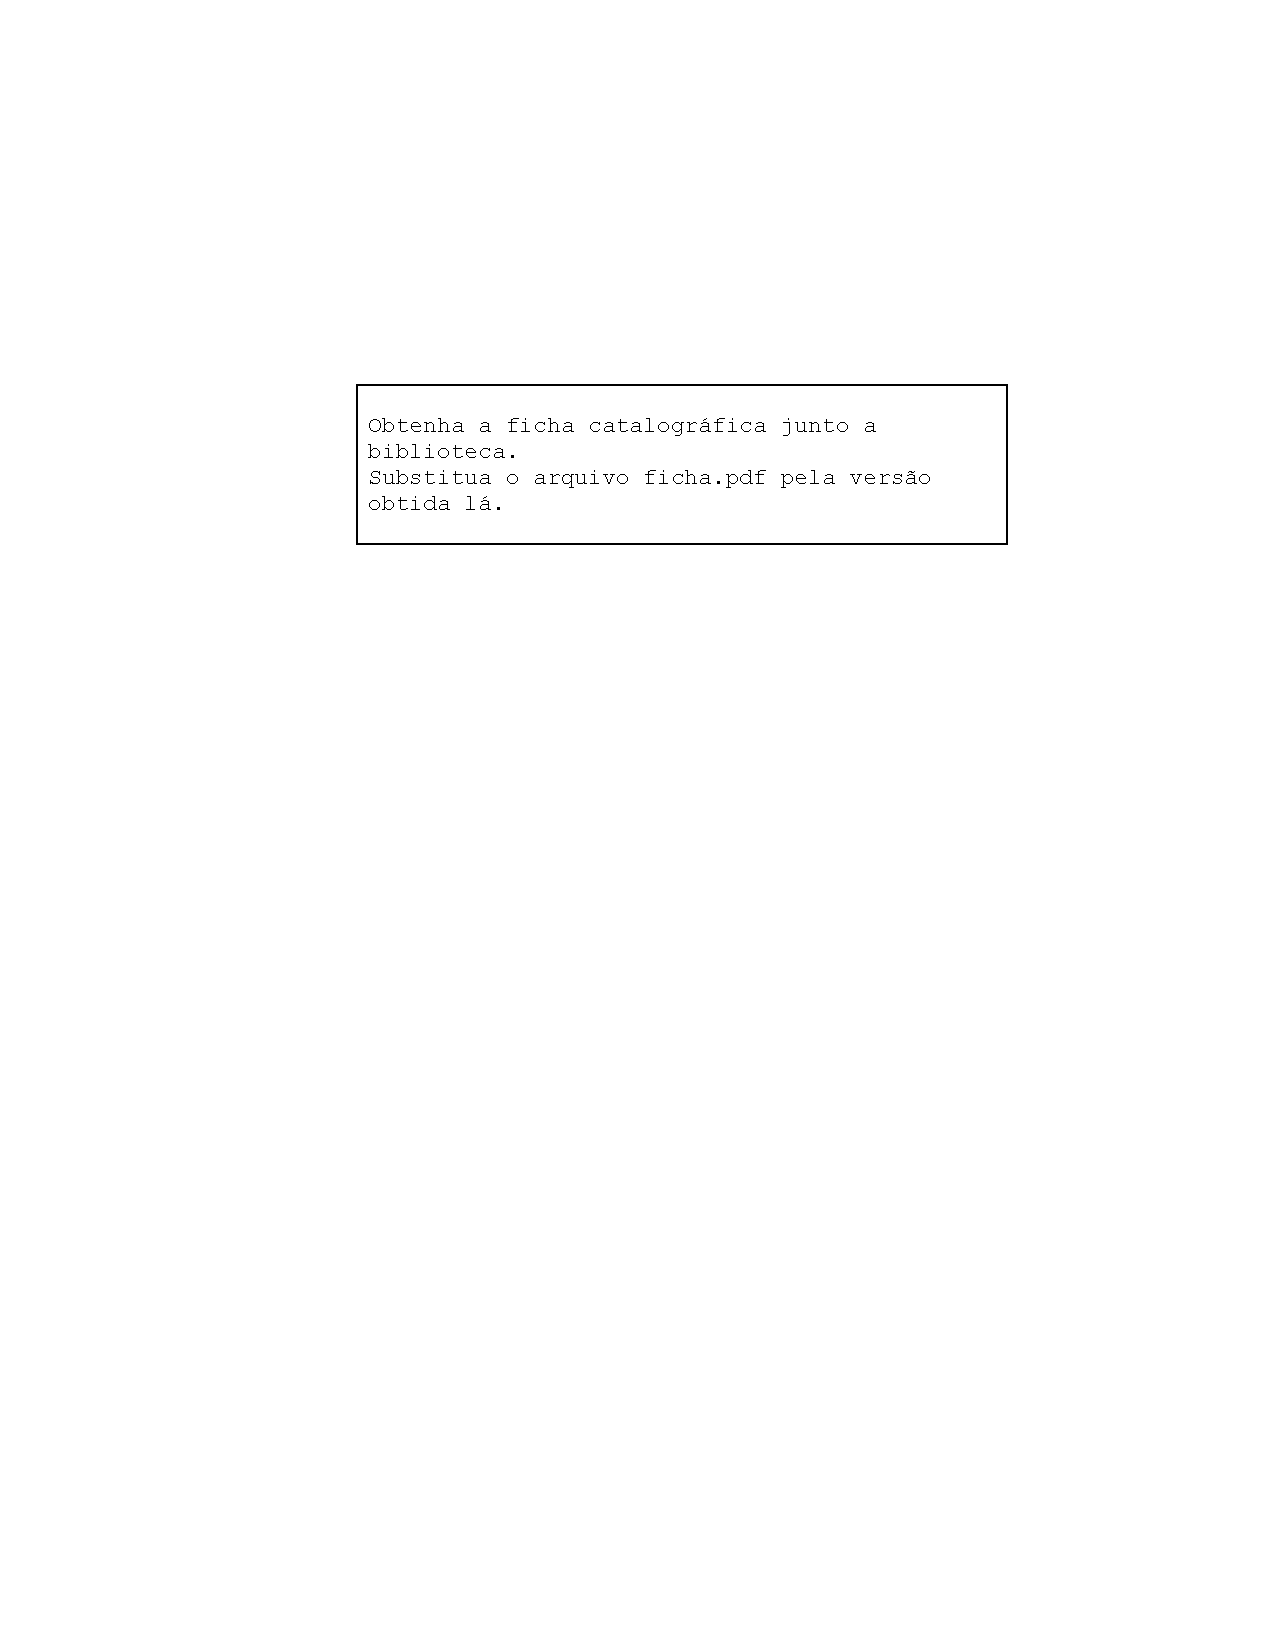
\includepdf{ficha.pdf}
\end{fichacatalografica}
% ---

% ---
% Inserir errata
% ---
% \begin{errata}
% Elemento opcional da \citeonline[4.2.1.2]{NBR14724:2011}. Exemplo:

% \vspace{\onelineskip}

% FERRIGNO, C. R. A. \textbf{Tratamento de neoplasias ósseas apendiculares com
% reimplantação de enxerto ósseo autólogo autoclavado associado ao plasma
% rico em plaquetas}: estudo crítico na cirurgia de preservação de membro em
% cães. 2011. 128 f. Tese (Livre-Docência) - Faculdade de Medicina Veterinária e
% Zootecnia, Universidade de São Paulo, São Paulo, 2011.

% \begin{table}[htb]
% \center
% \footnotesize
% \begin{tabular}{|p{1.4cm}|p{1cm}|p{3cm}|p{3cm}|}
%   \hline
%    \textbf{Folha} & \textbf{Linha}  & \textbf{Onde se lê}  & \textbf{Leia-se}  \\
%     \hline
%     1 & 10 & auto-conclavo & autoconclavo\\
%    \hline
% \end{tabular}
% \end{table}

% \end{errata}
% ---

% ---
% Inserir folha de aprovação
% ---

% Isto é um exemplo de Folha de aprovação, elemento obrigatório da NBR
% 14724/2011 (seção 4.2.1.3). Você pode utilizar este modelo até a aprovação
% do trabalho. Após isso, substitua todo o conteúdo deste arquivo por uma
% imagem da página assinada pela banca com o comando abaixo:
%
% \includepdf{folhadeaprovacao_final.pdf}
%
\begin{folhadeaprovacao}

  \begin{center}
    {\ABNTEXchapterfont\large\imprimirautor}

    \vspace*{\fill}\vspace*{\fill}
    \begin{center}
      \ABNTEXchapterfont\bfseries\Large\imprimirtitulo
    \end{center}
    \vspace*{\fill}
    
    \hspace{.45\textwidth}
    \begin{minipage}{.5\textwidth}
        \imprimirpreambulo
    \end{minipage}%
    \vspace*{\fill}
   \end{center}
        
%    Trabalho aprovado. \imprimirlocal, 24 de novembro de 2012:

   \assinatura{\textbf{\imprimirorientador} \\ Orientador} 
   \assinatura{\textbf{Professor} \\ Convidado 1}
   \assinatura{\textbf{Professor} \\ Convidado 2}
   %\assinatura{\textbf{Professor} \\ Convidado 3}
   %\assinatura{\textbf{Professor} \\ Convidado 4}
      
   \begin{center}
    \vspace*{0.5cm}
    {\large\imprimirlocal}
    \par
    {\large\imprimirdata}
    \vspace*{1cm}
  \end{center}
  
\end{folhadeaprovacao}
% ---

% ---
% Dedicatória
% ---
\begin{dedicatoria}
   \vspace*{\fill}
   \centering
   \noindent
   \textit{ Este trabalho é dedicado às crianças adultas que,\\
   quando pequenas, sonharam em se tornar cientistas.} \vspace*{\fill}
\end{dedicatoria}
% ---

% ---
% Agradecimentos
% ---
\begin{agradecimentos}
Os agradecimentos principais são direcionados à Gerald Weber, Miguel Frasson,
Leslie H. Watter, Bruno Parente Lima, Flávio de Vasconcellos Corrêa, Otavio Real
Salvador, Renato Machnievscz\footnote{Os nomes dos integrantes do primeiro
projeto abn\TeX\ foram extraídos de
\url{http://codigolivre.org.br/projects/abntex/}} e todos aqueles que
contribuíram para que a produção de trabalhos acadêmicos conforme
as normas ABNT com \LaTeX\ fosse possível.

Agradecimentos especiais são direcionados ao Centro de Pesquisa em Arquitetura
da Informação\footnote{\url{http://www.cpai.unb.br/}} da Universidade de
Brasília (CPAI), ao grupo de usuários
\emph{latex-br}\footnote{\url{http://groups.google.com/group/latex-br}} e aos
novos voluntários do grupo
\emph{\abnTeX}\footnote{\url{http://groups.google.com/group/abntex2} e
\url{http://abntex2.googlecode.com/}}~que contribuíram e que ainda
contribuirão para a evolução do \abnTeX.

\end{agradecimentos}
% ---

% ---
% Epígrafe
% ---
\begin{epigrafe}
    \vspace*{\fill}
	\begin{flushright}
		\textit{``Não vos amoldeis às estruturas deste mundo, \\
		mas transformai-vos pela renovação da mente, \\
		a fim de distinguir qual é a vontade de Deus: \\
		o que é bom, o que Lhe é agradável, o que é perfeito.\\
		(Bíblia Sagrada, Romanos 12, 2)}
	\end{flushright}
\end{epigrafe}
% ---

% ---
% RESUMOS
% ---

% resumo em português
% \setlength{\absparsep}{18pt} % ajusta o espaçamento dos parágrafos do resumo
% \begin{resumo}
%  Segundo a \citeonline[3.1-3.2]{NBR6028:2003}, o resumo deve ressaltar o
%  objetivo, o método, os resultados e as conclusões do documento. A ordem e a extensão
%  destes itens dependem do tipo de resumo (informativo ou indicativo) e do
%  tratamento que cada item recebe no documento original. O resumo deve ser
%  precedido da referência do documento, com exceção do resumo inserido no
%  próprio documento. (\ldots) As palavras-chave devem figurar logo abaixo do
%  resumo, antecedidas da expressão Palavras-chave:, separadas entre si por
%  ponto e finalizadas também por ponto.

%  \textbf{Palavras-chaves}: latex. abntex. editoração de texto.
% \end{resumo}

% resumo em inglês
% \begin{resumo}[Abstract]
%  \begin{otherlanguage*}{english}
%    This is the english abstract.

%    \vspace{\onelineskip}
 
%    \noindent 
%    \textbf{Key-words}: latex. abntex. text editoration.
%  \end{otherlanguage*}
% \end{resumo}
% ---

% ---
% inserir lista de ilustrações
% ---
% \pdfbookmark[0]{\listfigurename}{lof}
% \listoffigures*
% \cleardoublepage
% ---

% ---
% inserir lista de tabelas
% ---
% \pdfbookmark[0]{\listtablename}{lot}
% \listoftables*
% \cleardoublepage
% ---

% ---
% inserir lista de abreviaturas e siglas
% ---
% \begin{siglas}
%   \item[ABNT] Associação Brasileira de Normas Técnicas
%   \item[abnTeX] ABsurdas Normas para TeX
% \end{siglas}
% ---

% ---
% inserir lista de símbolos
% ---
% \begin{simbolos}
%   \item[$ \Gamma $] Letra grega Gama
%   \item[$ \Lambda $] Lambda
%   \item[$ \zeta $] Letra grega minúscula zeta
%   \item[$ \in $] Pertence
% \end{simbolos}
% ---

% ---
% inserir o sumario
% ---
\pdfbookmark[0]{\contentsname}{toc}
\tableofcontents*
\cleardoublepage
% ---



% ----------------------------------------------------------
% ELEMENTOS TEXTUAIS
% ----------------------------------------------------------
\textual

% ----------------------------------------------------------
% Introdução (exemplo de capítulo sem numeração, mas presente no Sumário)
% ----------------------------------------------------------
\chapter{Introdução}
% ----------------------------------------------------------

% introduzindo a jogos, por que é um mercado que está tao em alta
A indústria de jogos digitais cresce cada vez mais. De acordo com \citeonline{quanto_games_vao_movimentar}, essa indústria tende a ultrapassar em 2023, os US\$ 200 bilhões (aproximadamente, R\$ 1 trilhão). Novos jogos são produzidos e publicados diariamente, e somente na plataforma digital Steam, foram 10.644 novos títulos em 2022 como podemos ver na \cref{fig:steam_publishes} \space
% \cite{número_de_jogos_publicados_na_steam}.

\begin{figure}[!ht]
	\centering
    \caption{número de jogos publicados na Steam.}
	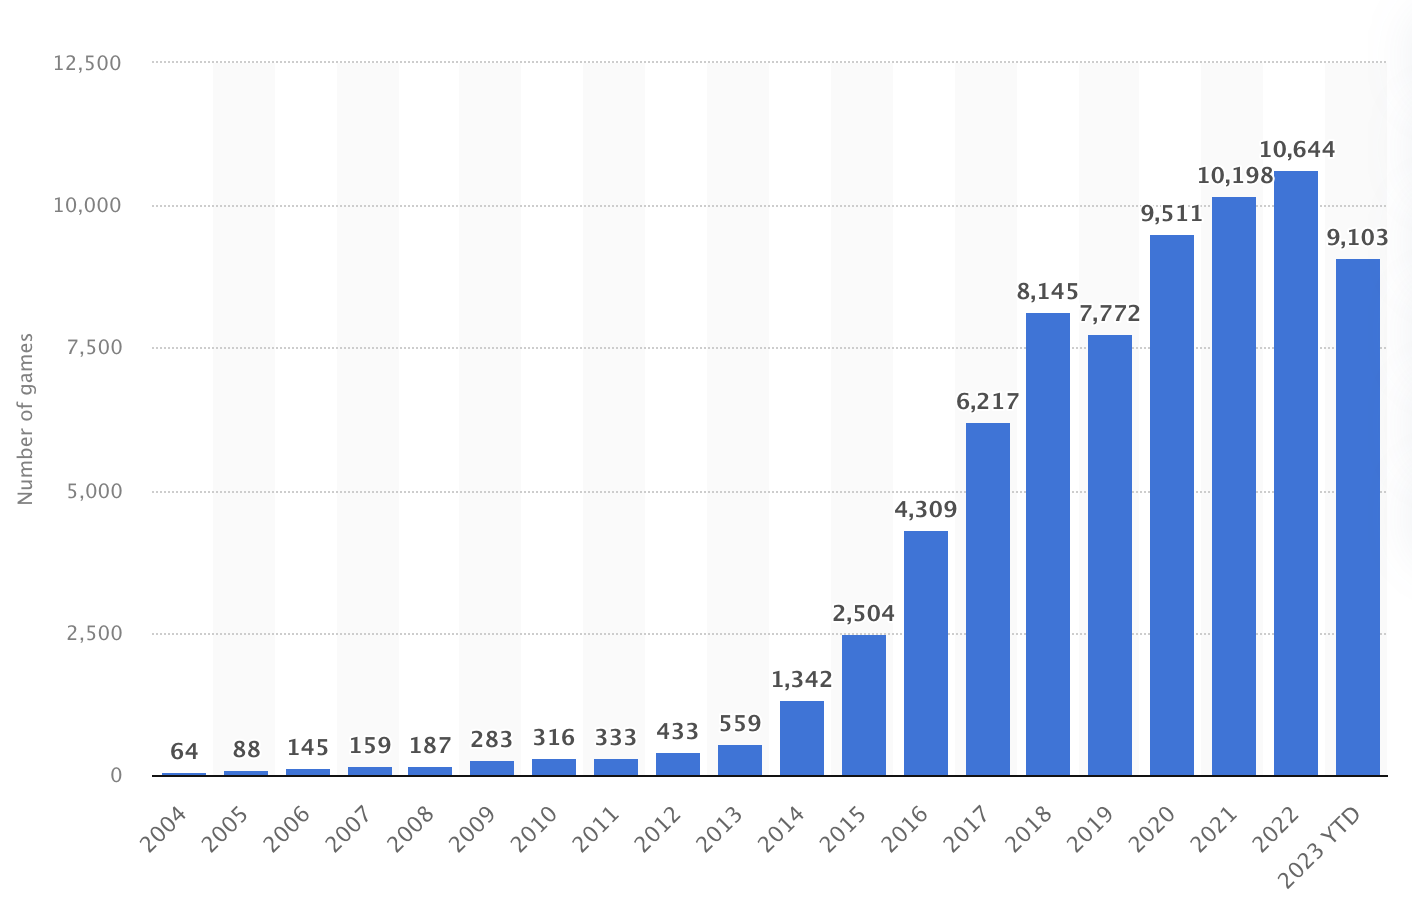
\includegraphics[width=0.6\textwidth]{figures/steam_sales.png}
	\legend{Fonte: \citeonline{numero_de_jogos_publicados_na_steam}}
	\label{fig:steam_publishes}
\end{figure}


% aqui a gente aproveita que falou de jogos para introduzir MAPAS que é o 'tema' do tcc
No cenário de jogos, os mapas desempenham um papel fundamental, fornecendo orientação aos jogadores e criando a sensação de escala em uma área. Por exemplo o jogo de aventura pirata chamado Sea of Thieves, os mapas revelam locais de interesse, como tesouros escondidos, missões e áreas perigosas, além de ajudar os jogadores a planejar suas estratégias, explorar o mundo virtual e tomar decisões com base em informações espaciais. Portanto os mapas enriquecem a experiência geral do jogo, mas cria-los pode ser um desafio, especialmente levando em consideração o orçamento disponível. Pois demandaria muitos recursos criar vários mapas diferentes com intuito de entretenimento do jogador. Em jogos como Minecraft, um elemento importante é a geração procedural, que consiste em um conjunto de algoritmos e ferramentas para geração de conteúdo, no qual se cria os mundos, com ilhas contendo biomas, cavernas, vilas, dentre outros recursos. Com essa diversidade de características pode-se evitar o tédio de sempre jogar no mesmo mapa \space\cite{video-game-maps, lecafedugeek}.

% \begin{figure}[ht]
% 	\caption{Mapa de tesouro do jogo Sea of Thieves}
% 	\centering % para centralizarmos a figura
% 	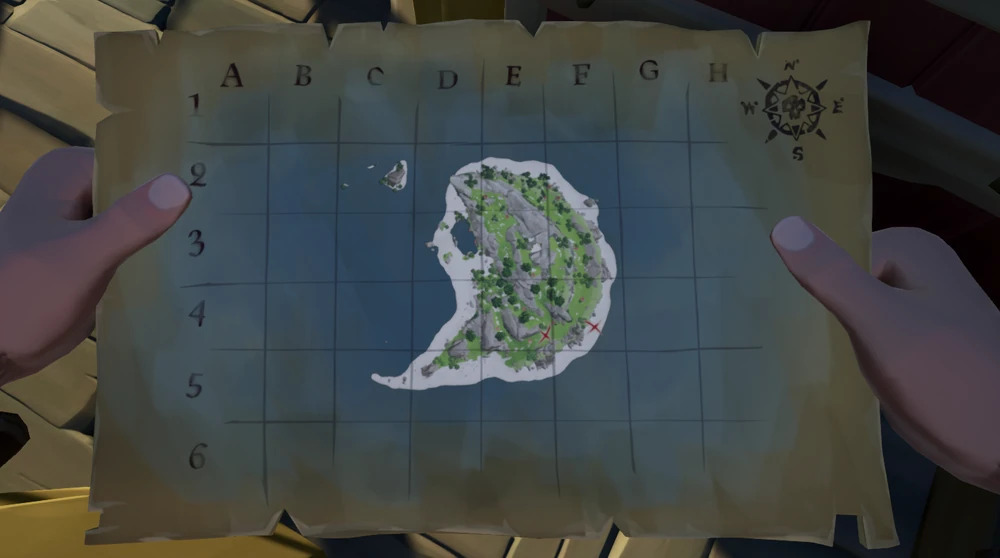
\includegraphics[width=10cm]{figures/Treasure_Map.jpg} % leia abaixo
% 	\legend{Fonte: \citeonline{seaofthieves}}
% 	\label{fig:treasureMap}
% \end{figure}

% aqui a gente faz um adendo e a demanda de jogos tende a crescer, então da a entender que você tem que produzir cada vez mais
% e também fala o quanto custa para produzir um jogo
% Ademais, o mercado de jogos no Brasil teve um aumento de 2,5\% em 2022, como apontado por uma pesquisa sobre o crescimento da demanda \space \space\cite{pesquisa_games_brasil}. O custo de produção de jogos varia bastante, dependendo do tamanho e da complexidade do projeto, \emph{e.g.}, a empresa Rockstar Games revelou que o jogo \textit{Grand Theft Auto V} custou cerca de 265 milhões de dólares para ser desenvolvido e comercializado \space \space\cite{gta_quanto_custou}.

%solução para o problema
% Apesar do rápido crescimento da indústria, existe uma carência de ferramentas que possam auxiliar os designers e artistas durante o processo de produção de jogos, o que acaba tornando-o demorado e, consequentemente, mais caro.  Segundo o livro "Procedural Content Generation in Games" \space\cite{procedural_centent_book}, uma abordagem eficiente para reduzir os custos de produção de um jogo é utilizar a geração procedural de conteúdo. Essa técnica permite maximizar o desenvolvimento de um jogo, envolvendo o uso de um software de computador capaz de criar conteúdo de jogos automaticamente. Esse software possibilita a geração automatizada de mapas, otimizando o processo de desenvolvimento.


% No entanto, a criação de mapas usando esse método ainda encontram dificuldades, sendo elas, variedade e autenticidade \space\cite{geracao_procedural_jogos_2d}.
% aqui adicionar uma explicação do porque é um desafio a geração procedural de conteúdo

Contextualizando, a área de Geometria Computacional é um ramo da ciência da computação que estuda algoritmos e estruturas de dados, servindo para resolução computacional de problemas geométricos. O diagrama de Voronoi é um dos tópicos mais discutidos dessa
área e possui uma gama de utilizações, dentre elas pode ser utilizado para resolver alguns problemas relacionados a jogos como por exemplo marcar pontos no mapa, desses pontos criar regiões, e a partir dessas regiões criar biomas gerando um mapa \space\cite{rodrigues_diagrama_2019}.


% introduz a relação de ia para personalização dentro de métodos procedurais em jogos
De acordo com \citeonline{jogo_procedural} é muito comum usar técnicas procedurais combinado com Inteligência Artificial (IA) para melhorar ou personalizar a experiência do jogador. Por exemplo, o jogo RimWorld é um simulador de colônia que gera um planeta de forma procedural e utiliza uma IA para narrar a história, abrangendo psicologia, ecologia, combate e diplomacia, dentre outros. Logo, essa combinação entre IA e a geração procedural cria uma jogabilidade única ao jogador.

% A aplicação da IA em jogos não se limita apenas à jogabilidade. Ela também é usada em áreas como animação de personagens, reconhecimento de fala e expressões faciais, tradução automática de idiomas nos diálogos do jogo e muito mais. A IA está impulsionando a inovação e a evolução dos jogos, proporcionando experiências cada vez mais envolventes e cativantes para os jogadores \space\cite{exameNvidia, omniverseace}.

% introduz o ramo de segmentação geral que será explicado mais para frente
Em IA, um ramo que está em ascensão é o de segmentação de imagem com redes neurais convolucionais, que constitui-se em classificar os pixeis de uma imagem ou criar áreas na imagem para destacar cada objeto (todas classes que são contáveis como pessoas, carros, etc) detectado ou até mesmo mesclar essas duas técnicas. Neste ramo existem diversas aplicações, como por exemplo carros autônomos e sistemas de vigilância.
Na aplicação de carros autônomos é necessário identificar humanos para tomar decisões de freio, em sistemas de vigilância é necessário identificar para alertar e automatizar o processo de segurança. Portanto, nessas aplicações reais observa-se a importância em identificar seres humanos para a tomada de decisões \space\cite{dp_semantic_segmantation}.

% Nessas aplicações é possível observar que é preciso ter um foco em identificar e segmentar seres humanos, por exemplo, em carros autônomos é primordial essa tarefa para o carro tomar a decisão de frear quando estiver muito perto de bater.

% Logo, se torna um tópico relevante dentro de visão computacional, no qual pode ter diversas aplicações no mundo real \space\cite{kirillov2019panoptic, dp_semantic_segmantation}.

Com base na contextualização é possível perceber que o mercado de jogos está em ascensão, o mapa é um recurso importante e pode ser usado a técnica de geração procedural para diversificar, o diagrama de Voronoi pode ser usado para gerar biomas em mapas no processo de geração procedural, a técnica de geração procedural de conteúdo unido a inteligência artificial é muito utilizado em jogos para criar personalizações, no ramo de inteligência artificial a segmentação com redes neurais convolucionais está em destaque. Logo pode-se perceber a relevância desses temas no curso de ciência da computação e na atualidade, propõe-se então, uma solução para personalizar mapas de jogos utilizando um modelo de IA da área de segmentação usando redes neurais convolucionais.

Com o objetivo de gerar mapas com biomas de forma procedural com personalização de IA, decidiu-se utilizar o resultado da segmentação de imagem por rede neural convolucional para o usuário selecionar uma área e assim delimitar o contorno da ilha, adicionando, portanto, uma personalização. Essa aplicação possibilita um desenvolvedor de jogos criar um protótipo de mapa rapidamente ou aprimorar e usar esse recurso no jogo, possibilitando o jogador tirar ou selecionar uma foto e escolher um contorno para gerar um mapa com aquele formato.

Por fim, para contribuição científica tem-se a hipótese de que quanto mais pontos o diagrama de Voronoi tiver maior será a precisão da compatibilidade entre o mapa gerado e o contorno escolhido. Para chegar a essa conclusão, comprometeu-se definir alguns testes com métricas em prol de mensurar a qualidade da geração procedural com o contorno selecionado.


% Por conseguinte, a combinação entre inteligência artificial e geração procedural de mapas pode abrir novas possibilidades de personalização nos jogos. Imagine um jogo em que, a partir da segmentação de imagens por meio de redes neurais convolucionais, os jogadores possam criar mapas únicos e personalizados para suas aventuras. Com uma foto, o modelo treinado segmentaria a imagem para selecionar um contorno reconhecido, e a partir dele se criar um mapa de maneira procedural contendo biomas no mesmo formato escolhido.

% No contexto da geração procedural de mapas, explorar a relação entre IA e personalização de jogos contribuirá para o avanço dessas áreas de pesquisa, proporcionando aos jogadores experiências mais ricas e variadas.

% Adicionar uma parte explicando a parte de visão computacional e porque o tema da nossa Ia é identificação de pessoas

% Dito isso, nosso projeto tem a ideia de fornecer recursos baseados em matemática aplicada dentro de ciência da computação que proporcione uma funcionalidade de escolher o contorno do mapa no qual irá jogar através de imagens. Abordaremos a arquitetura de redes neurais convolucionais, que é muito utilizada para trabalhar com imagens. Mais especificamente, abordaremos uma arquitetura derivada da arquitetura mencionada anteriormente, específica para segmentação de imagens, o que possibilita classificar contornos em imagens.

\section{Objetivos}

O objetivo principal deste trabalho é desenvolver uma ferramenta que ofereça uma alternativa para a geração procedural de mapas de ilhas, utilizando o diagrama de Voronoi para a criar biomas. Além disso, pretende-se combinar segmentação com redes neurais convolucionais para permitir a personalização desses mapas. Essa ferramenta terá a capacidade de reconhecer os contornos reconhecidos (classificados no conjunto de dados, logo o resultado terá uma detecção abrangente dentro do escopo de classes obtidas) de uma imagem, e gerar um mapa com um mapa baseado nos limites do contorno escolhido.

Adicionalmente, os seguintes objetivos específicos serão abordados:

\begin{itemize}
	\item Selecionar e analisar conjuntos de dados contendo classes relevantes, como pessoas, carros, entre outros, para treinar um modelo de rede neural convolucional específico para segmentação de imagens.
	\item Utilizar algoritmos para criar diagramas de Voronoi.
	\item Aplicar um algoritmo para reconhecer a imagem com o contorno selecionado e gerar como resultado a imagem do mapa gerado.
	\item Utilizar o resultado da segmentação para selecionar indicar o que é terreno em cima do diagrama de Voronoi.
	\item Gerar os biomas no diagrama de Voronoi.
	\item Criar testes em prol de mensurar a semelhança entre o contorno do mapa gerado com o contorno escolhido.
\end{itemize}

% Outro cenário que está crescendo muito nos últimos anos é o da inteligência artificial, afirma \citeonline{Valente_2020} que no Brasil mais que dobrou o número contratações de desenvolvedores da área de 2015 até 2020. De acordo com \apud{johnson2023}{briggs2023} um relatório recente relata que 300 milhões de empregos podem ser afetados pela IA \emph{i.e.} 18\% ofício global pode ser automatizado. Outrossim \citeonline{europarl2020} diz que o tópico de inteligência artificial é uma prioridade para União Europeia por ser considerada primordial para transformação digital da sociedade.  Do mesmo modo, Bill Gates, um dos fundadores da Microsoft — uma das maiores empresas de tecnologia —, diz que "o desenvolvimento da inteligência artificial (IA) é o avanço tecnológico mais importante em décadas"\space
% \space\cite{inteligencia_artificial_e_avanco_bbc}.

\chapter{Fundamentação teórica}
\label{sec:background}
	\label{sec:fund_teorica}

Este capítulo tem objetivo de apresentar conceitos necessários para entendimento do trabalho.

\section{Visão computacional}

A visão computacional está em constante avanço, aproximando cada vez mais os computadores da capacidade visual humana. De acordo com Horst Haußecker e Bernd Jähne, no livro "Computer Vision and Applications" \cite{comp_vision_and_applications}, a visão computacional é uma área da computação que se dedica à interpretação de imagens por meio de algoritmos e técnicas de processamento de imagens. Essa área abrange a aquisição, processamento e análise de imagens, com o objetivo de extrair informações úteis para resolver problemas específicos.

Porém, segundo Richard Szeliski, no livro "Computer Vision: Algorithms and Applications" \cite{computer_vision_richard}, nas últimas décadas ocorreram avanços significativos na busca de aproximar a visão computacional da visão humana, porém não obteve total êxito. Isso ocorre porque, enquanto o olho humano enxerga com aparente facilidade as estruturas tridimensionais e suas nuances, a visão computacional depende de técnicas matemáticas altamente precisas para recuperar a forma tridimensional e a aparência dos objetos.

Nas figuras \cref{fig:imagem_a} e \cref{fig:imagem_b}, evidencia-se a notável capacidade de um computador em distinguir, classificar e até mesmo compreender os elementos presentes em uma fotografia.

\begin{figure}
    \centering
    \begin{minipage}[b]{0.49\textwidth}
      \centering
      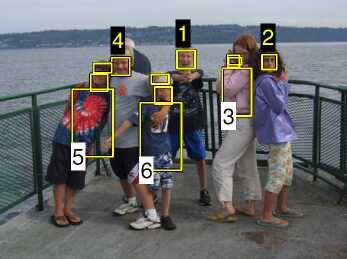
\includegraphics[width=0.6\textwidth]{figures/detectacao_de_faces_exemplo.JPG}
      \caption{Algoritmos de detecção facial e de roupas/cabelos por cor localizam e reconhecem pessoas nesta imagem \cite{computer_vision_richard}}
      \label{fig:imagem_a}
    \end{minipage}
    \hfill
    \begin{minipage}[b]{0.49\textwidth}
      \centering
      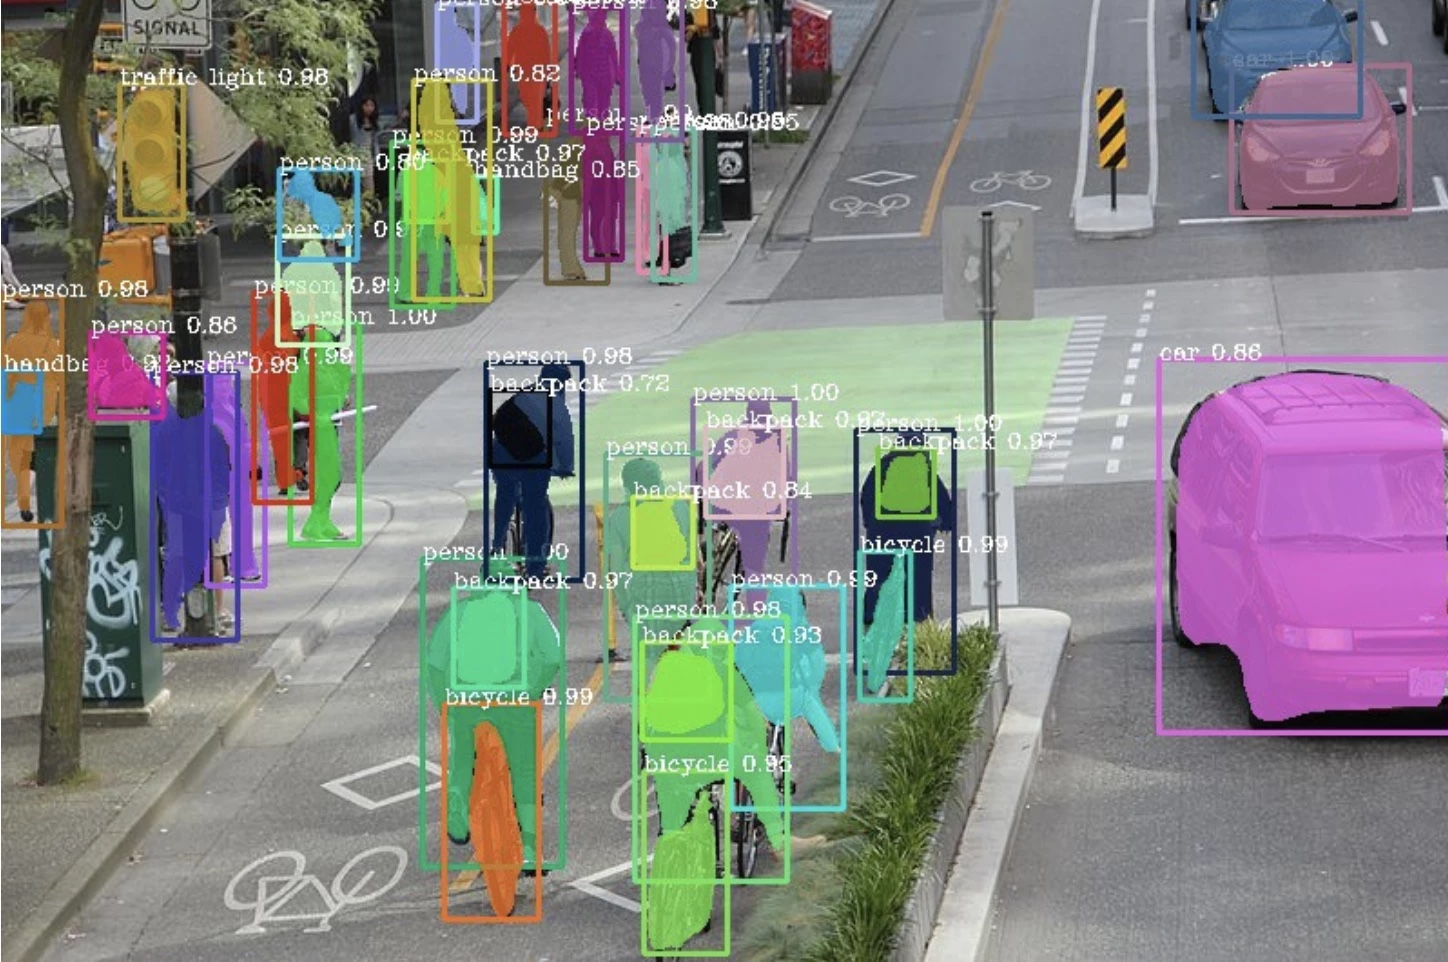
\includegraphics[width=0.6\textwidth]{figures/semantic_intance.JPG}
        \caption{Segmentação de instâncias de objetos pode delinear cada pessoa e objeto em uma cena complexa. 
        \cite{instance_segmentation}}
      \label{fig:imagem_b}
    \end{minipage}
  \end{figure}


No entanto, apesar do sucesso no uso dessas técnicas, o computador ainda não consegue oferecer a mesma quantidade de detalhes na explicação de uma imagem como o olho humano. Isso se deve à maior facilidade do computador em compreender linguagem em comparação à visualização. A tarefa de ensinar um computador a ver e descrever com precisão e riqueza de detalhes o que está sendo observado é extremamente complexa \cite{computer_vision_richard}.

A visão é um elemento crucial para capacitar a inteligência artificial a realizar diversas tarefas. A fim de replicar a visão humana, é necessário que as máquinas sejam capazes de adquirir, processar, analisar e compreender imagens. \cite{como_funciona_visao_computacional}

% Na \cref{fig:comp_vision} podemos ver uma analogia entre a forma como uma imagem é processada pelo cérebro humano e a forma como é processada por um sistema computacional.

% \begin{figure}[!ht]
% 	\centering
% 	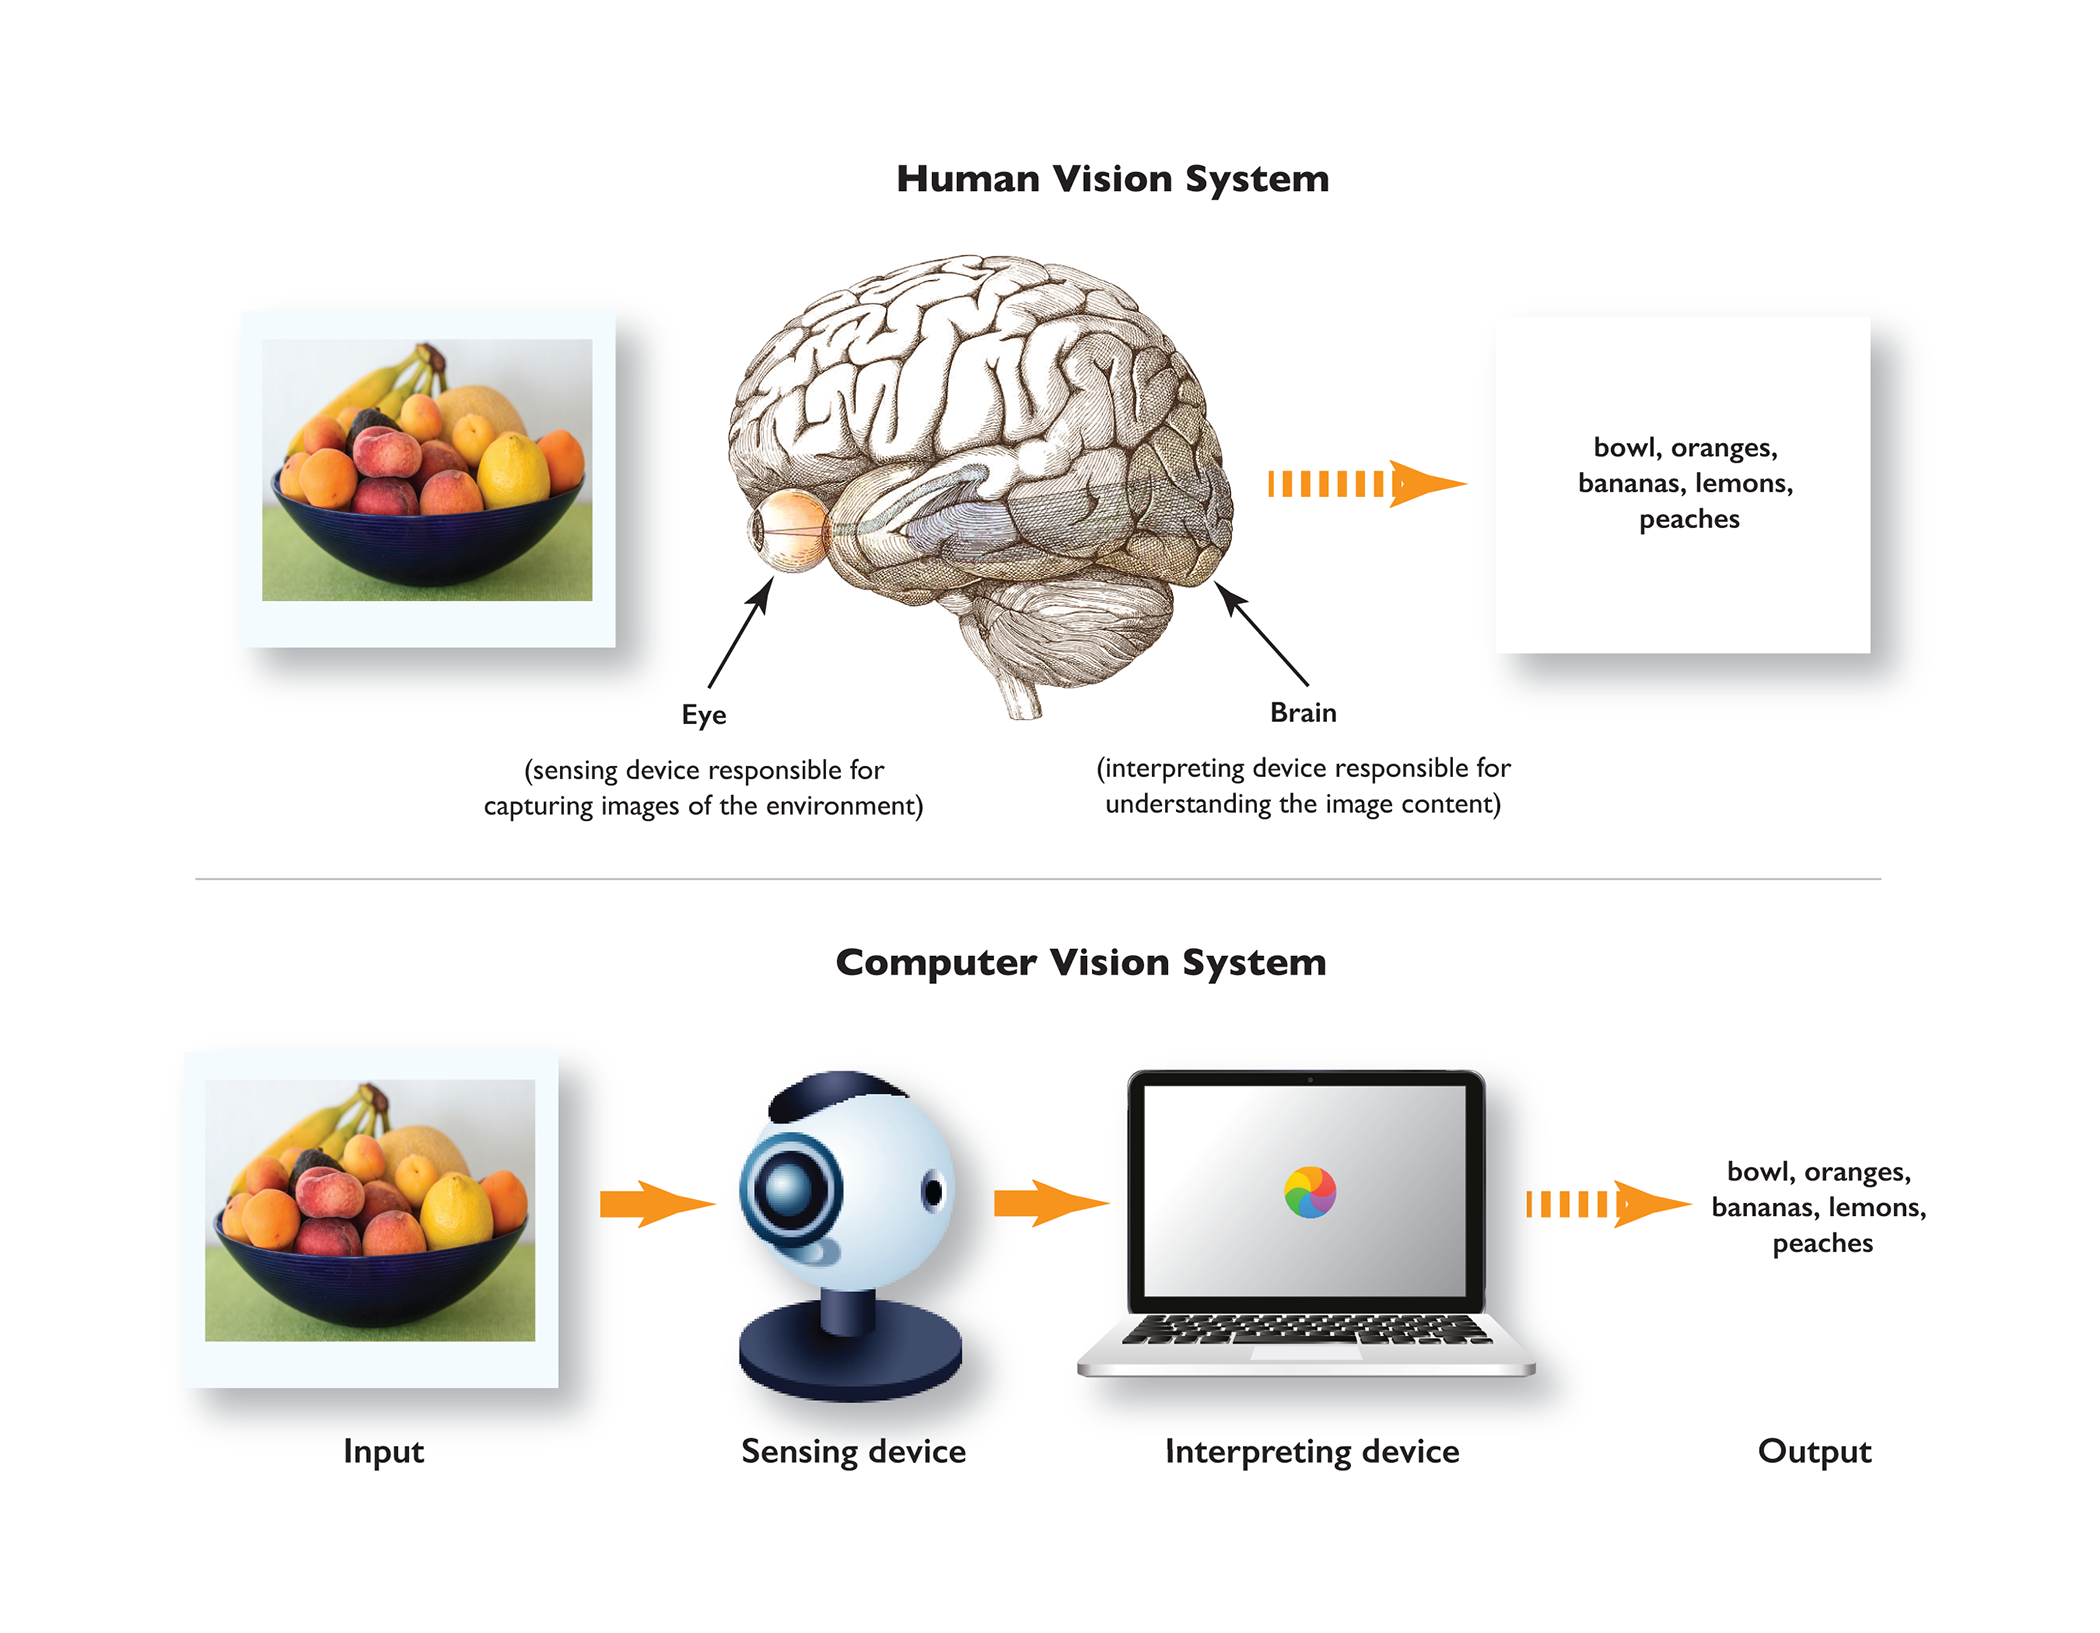
\includegraphics[width=0.6\textwidth]{figures/content_Human_Vision.png}
% 	\caption{Visão humana e sistemas de visão computacional processam dados visuais de maneira semelhante \cite{content_Human_Vision}.}
% 	\label{fig:comp_vision}
% \end{figure}	

No processamento de computação visual, as imagens são adquiridas e representadas como uma matriz 2D de pixels. Cada pixel corresponde a um ponto na imagem e é representado por um valor numérico que varia de 0 a 255. Esses valores de pixel descrevem a intensidade da cor em uma escala de cinza. Dessa forma, um computador interpreta uma imagem como uma matriz de números, permitindo que ele analise e compreenda os detalhes visuais presentes na imagem, como no caso da \cref{fig:comp_vision} do presidente dos Estados Unidos, Abraham Lincoln\cite{mit_video}.

Os algoritmos de visão computacional utilizados atualmente são fundamentados em reconhecimento de padrões. O procedimento consiste em treinar computadores por meio de uma vasta quantidade de dados visuais. Os computadores processam imagens, rotulam os objetos nelas contidos e identificam padrões entre esses objetos \cite{content_Human_Vision}.

Esse processo de treinamento e reconhecimento de padrões permite que os computadores identifiquem objetos e compreendam seu contexto visual. Com essa capacidade, o computador consegue realizar tarefas como, por exemplo, reconhecimento facial \cref{fig:imagem_a}.

\begin{figure}[!ht]
	\centering
	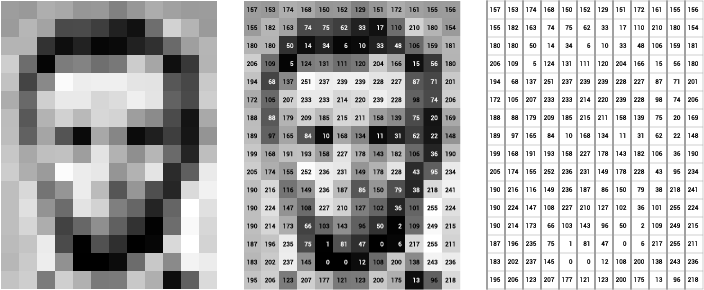
\includegraphics[width=0.6\textwidth]{figures/lincoln_pixel_values.png}
	\caption{Diagrama de dados de pixels. À esquerda, nossa imagem de Lincoln; no centro, os pixels rotulados com números de 0 a 255, representando sua luminosidade; e à direita, apenas esses números \cite{content_Human_Vision}.}
	\label{fig:comp_vision}
\end{figure}





\section{Inteligência Artificial}
Inteligência artificial é uma técnica científica que simula o pensamento humano de forma que possa ser executado em uma máquina, podendo ser utilizada para criar soluções com uma linha de progressão parecida ao raciocínio lógico como conhecemos. Isto permite ao computador reconhecer e interpretar o mundo ao redor com imagens e textos criando uma ampla área de atuação que otimiza tarefas antes só realizadas por seres humanos \space\cite{ia_aliada_ou_inimiga}.

Este ramo é complexo por se tratar de uma representação cognitiva, se torna necessário usar uma base com diversas áreas científicas como psicologia, biologia, lógica matemática, linguística, engenharia, filosofia, entre outras. E pode ser usado para diversos problemas específicos como, por exemplo, definir as boas rotas para algum processo logístico \space\cite{ia_conceitos_aplicacoes}.

\begin{figure}[H]
	\caption{Diagrama de aprendizado de máquina}
	\centering % para centralizarmos a figura
	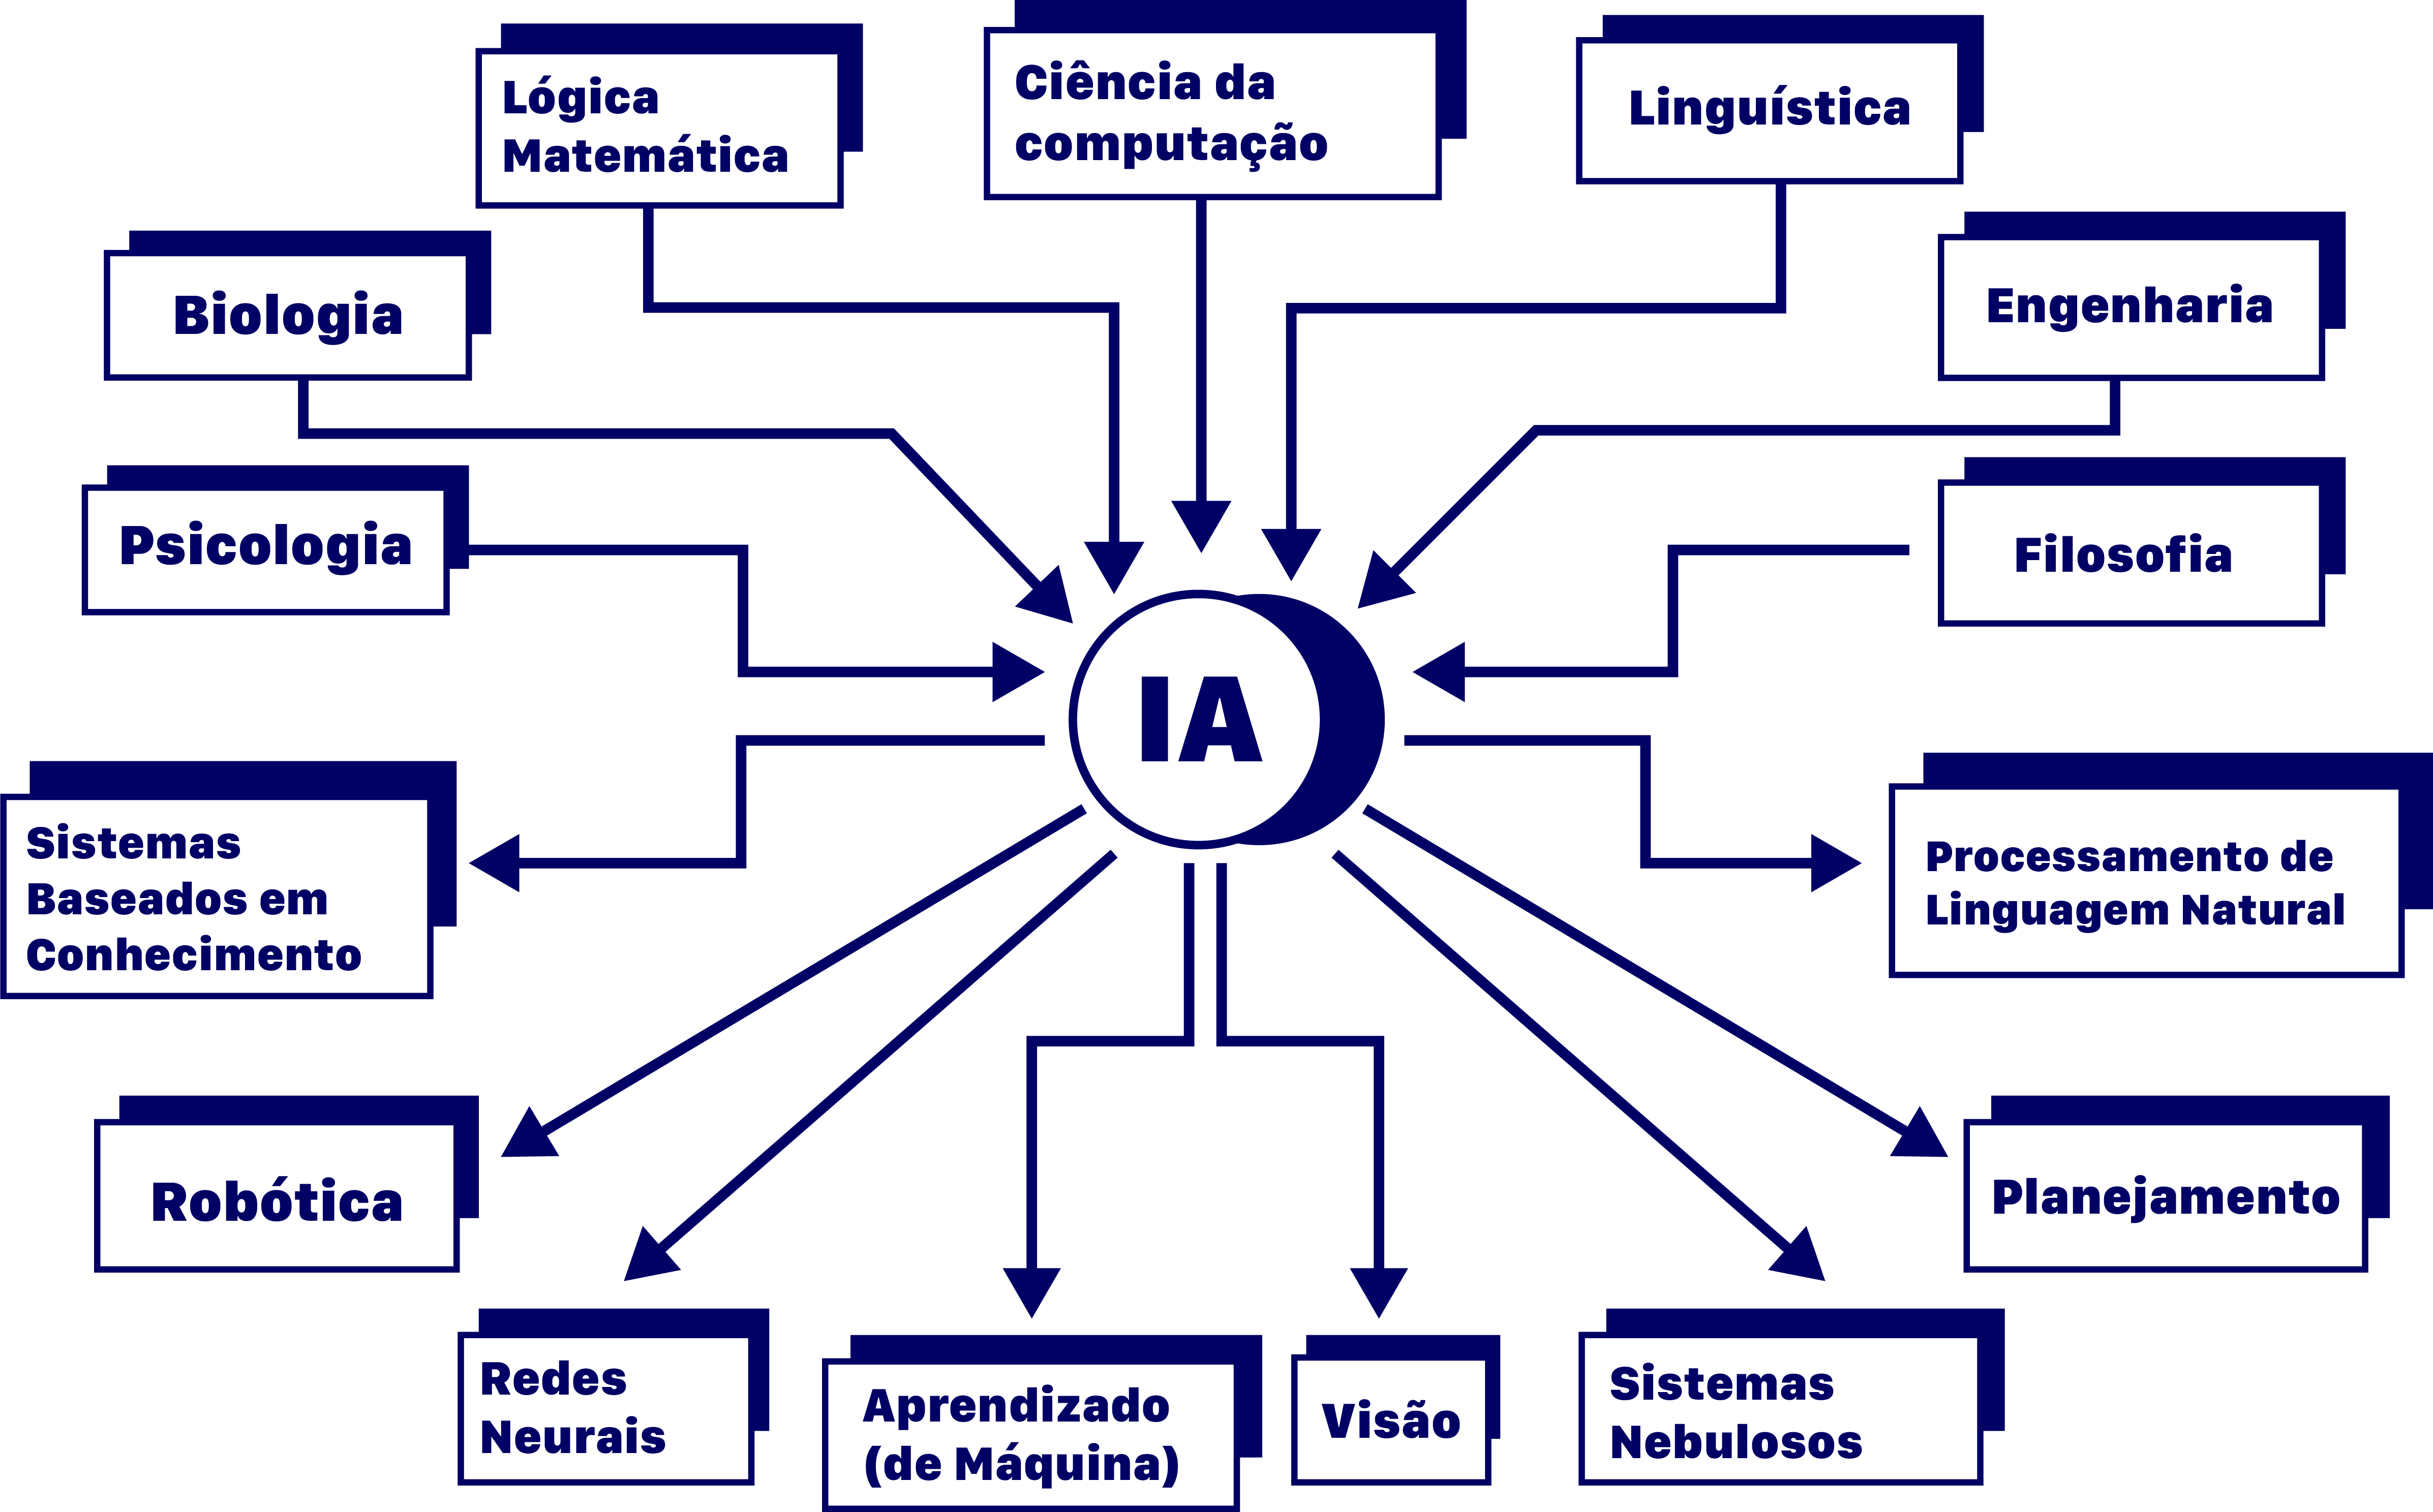
\includegraphics[width=10cm]{figures/areas_ia.png} % leia abaixo
	\legend{Fonte: \citeonline{aplicacoes_ia_vg}}
	\label{fig:areas_ia}
\end{figure}

Segundo \citeonline{dp_overview} existe três tópicos sobre inteligência artificial muito populares sendo eles, inteligência artificial, aprendizado de máquina e aprendizado profundo como segue na imagem \cref{fig:diagrama_ia_ml_dp}.

\begin{figure}[H]
	\caption{Diagrama de Venn sobre relação entre os tópicos de inteligência artificial}
	\centering % para centralizarmos a figura
	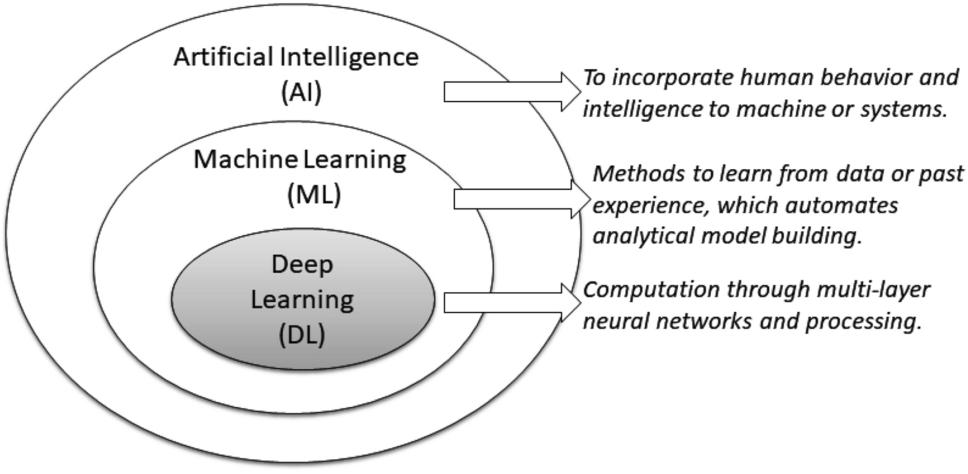
\includegraphics[width=10cm]{figures/diagrama_ia_ml_dp.png} % leia abaixo
	\legend{Fonte: \citeonline{dp_overview}}
	\label{fig:diagrama_ia_ml_dp}
\end{figure}



\subsection{Aprendizado de Máquina}

Segundo \citeonline{directions_ia_ml_dp}, aprendizado de máquina é uma subcategoria de inteligência artificial que se refere  a detecção de padrões importantes de uma base de dados. As ferramentas utilizadas aumentam a eficiência dos algoritmos para lidar com bases de dados grandes.

Portanto, essa técnica permite ao computador melhorar os resultados com base na experiência, isso indica uma relação direta entre o quanto o programa consumiu de dados e qualidade da solução do problema \cite{ml_explicado}. 

Dentro desse nicho existem outros como: redes neurais, algoritmos evolucionários, algoritmos de busca, aprendizado por reforço, dentre outros. \cite{ml_oil_gas_industry}.

É possível observar uma hierarquia entre aprendizado de máquina e os principais termos, sendo eles: redes neurais artificiais e aprendizado profundo com base em \citeonline{ml_and_dp} mostrado na ilustração da \cref{fig:diagrama_ann}. Esses termos são importantes para compreensão geral da área de segmentação contida em redes neurais.

\begin{figure}[H]
	\caption{Ilustração da relação entre os principais tópicos de aprendizado de máquina}
	\centering % para centralizarmos a figura
	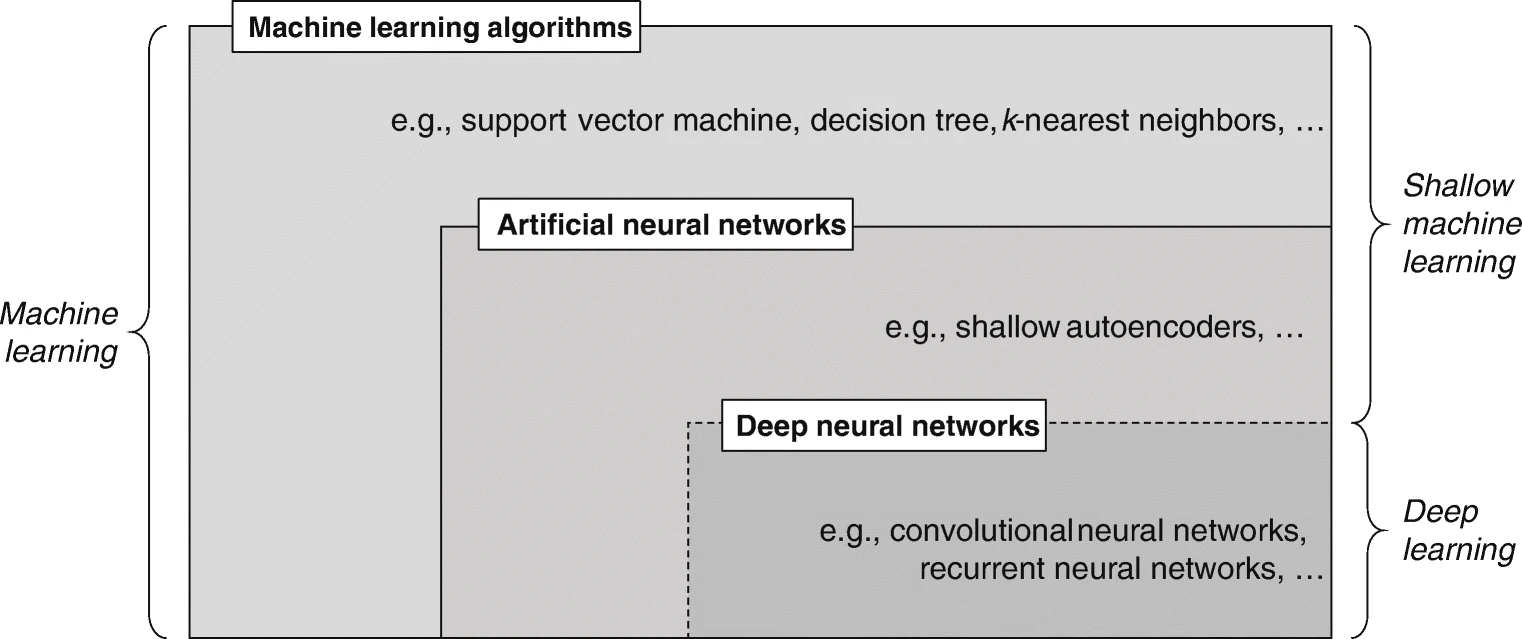
\includegraphics[width=10cm]{figures/diagrama_ann.jpg} % leia abaixo
	\legend{Fonte: \citeonline{ml_and_dp}}
	\label{fig:diagrama_ann}
\end{figure}


\subsubsection{Rede neural artificial}

Uma rede neural artificial é uma representação matemática de unidades de processamento conectadas chamadas de neurônios artificiais . Essa arquitetura simula sinapses, cada sinal trocado entre os neurônios pode aumentar ou atenuar os sinais de outros durante o aprendizado\cite{ml_and_dp}.
\begin{figure}[H]
	\centering
	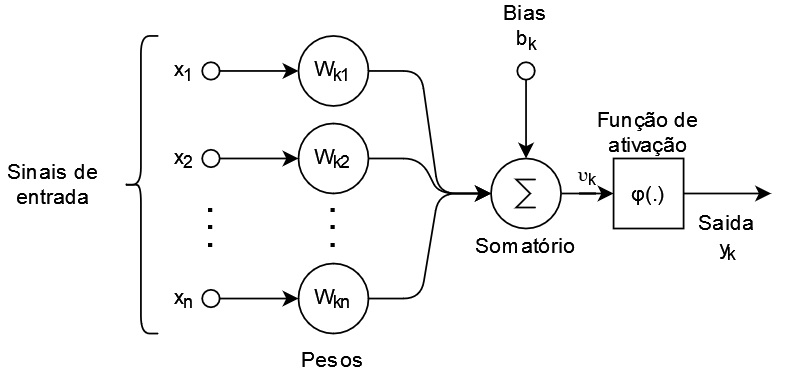
\includegraphics[width=0.8\textwidth]{figures/neuronio.png}
	\caption{Modelo de um neurônio não-linear \cite{haykin1999neural}.}
	\label{fig:neuronio}
\end{figure}

Observando a figura \ref{fig:neuronio} vemos o funcionamento de um neurônio $k$. Os sinais de entradas são partes de um vetor $x$ de tamanho $n$, sendo o vetor composto por $x_1, x_2 ... x_n$. Essas componentes são combinadas em uma soma ponderada utilizando seus respectivos pesos, $w_{k1}, w_{k2}...w_{kn}$, formando assim a seguinte equação  \apud{marti2017aprendizado}{haykin1999neural}:

$$\upsilon_k = \sum_{i=1}^n (x_i * w_{ki})$$

O resultado dessa equação produz o potencial de ativação $\upsilon_k$, esse resultado é somado com o \textit{bias} ou viés $b_k$ para manipular a saída $y_k$ do neurônio, essa soma é posta em uma função não-linear nomeada de função de ativação $\varphi(.)$, essas funções mapeiam a saída em um intervalo $[0, 1]$ ou $[1, -1]$. A função de saída pode ser representada com a seguinte equação \apud{marti2017aprendizado}{haykin1999neural}:

$$y_k = \varphi(\upsilon_k + b_k)$$

O aprendizado ocorre na fase de treinamento onde é ajustando os pesos $w_k$ e o viés $b_k$ de cada neurônio $k$. Os pesos $w_k$ são utilizados para calcular a taxa de crescimento da função e o viés $b_k$ é necessário para descolar a saída da função. Com isso é possível modelar uma função linear $y=w^T*x+b$ \cite{marti2017aprendizado}.

Para cada amostra o modelo compara os resultados dos valores atuais dos pesos $w_k$ e viés $b_k$ com o resultado esperado(alvo). Uma função custo(\textit{cost function}) é utilizada para gerar um vetor de gradientes e para quantificar o erro encontrado para a configuração atual do modelo. O modelo atualiza os pesos $w_k$ e os viés $b_k$ no sentido contrário do vetor de gradientes, buscando minimizar a função de custo de acordo com uma taxa de aprendizado(\textit{learning rate}) \cite{marti2017aprendizado}.

Ao combinar diversos neurônios artificiais forma-se uma rede neural Artificial. Essas redes buscam simular o processamento de informação do cérebro humano \cite{ferneda2006redes}.
Nas redes neurais os neurônios são organizados em grupos de unidade de processamento chamados camadas. A primeira e a última camada são nomeadas de camada de entrada e camada de saída e as demais de camadas ocultas. As camadas mais próximas da entrada são responsáveis por identificar características mais primitivas e as seguintes combinam essas informações para identificar padrões mais complexos \cite{marti2017aprendizado}.


\subsubsection*{Função de ativação}

A função de ativação retorna a saída de um neurônio \space\cite{haykin1999neural}, aqui pode-se ver quatro tipos de funções de ativação:

\begin{enumerate}
	\item Função \textit{Sigmoid}, uma função não-linear que produz uma curva com a forma de "S". Usada para mapear valores previstos em probabilidades. Tem o valor de saída entre 0 e 1 \space\cite{gharat2019what}.
	\begin{figure}[ht]
	\caption{Gráfico da função \textit{Sigmoid}.}
	\begin{center}
		\begin{minipage}{0.45\textwidth}
			\begin{equation}
				\varphi(\upsilon) = \frac{1}{1 + e^{-\upsilon}}
			\end{equation}
		\end{minipage}
		\hfill
		\begin{minipage}{0.45\textwidth}
			\begin{tikzpicture}
				\begin{axis}[
					width=0.9\textwidth,
					height=0.7\textwidth,
					xmin=-10, xmax=10,
					ymin=-0.2, ymax=1,
					xtick=\empty,
					ytick=\empty,
					axis lines=middle,
					xlabel={$\upsilon$},
					ylabel={$y$},
				]
					\addplot[blue,domain=-10:10,samples=51] {1/(1+exp(-x))};
				\end{axis}
			\end{tikzpicture}
		\end{minipage}
	\end{center}
	\legend{Fonte: Criação própria}
	\label{fig:grafico_sigmoid}
	\end{figure}
	Segundo \citeonline{gharat2019what}, a função \textit{Sigmoid} tem uma convergência lenta, é computacionalmente cara e para valores muito extremos causa problemas na previsão.

	\item Função \textit{ReLu} (Unidade Linear Retificada), função não-linear inspirada nos neurônios do cérebro que retorna um valor positivo ou 0 \space\cite{rizzo2020inteligencia}.
	\begin{figure}[ht]
	\caption{Gráfico da função \textit{ReLu}.}
	\begin{center}
		\begin{minipage}{0.45\textwidth}
			\begin{equation}
				\label{eq:relu_func}
				\varphi(\upsilon) = \max(0,\upsilon)
			\end{equation}
		\end{minipage}
		\hfill
		\begin{minipage}{0.45\textwidth}
			\begin{tikzpicture}
				\begin{axis}[
					width=0.9\textwidth,
					height=0.7\textwidth,
					xmin=-2, xmax=2,
					ymin=-0.5, ymax=2,
					xtick=\empty,
					ytick=\empty,
					axis lines=middle,
					xlabel={$\upsilon$},
        			ylabel={$y$},
				]
					\addplot[line width=1pt,color=blue,domain=-2:0] plot(\x,{0});
					\addplot[line width=1pt,color=blue,domain=0:2] plot(\x,{\x});
				\end{axis}
			\end{tikzpicture}
		\end{minipage}
	\end{center}
	\legend{Fonte: Criação própria}
	\label{fig:grafico_relu}
	\end{figure}
	A função \textit{ReLu} é computacionalmente eficiente e converge rapidamente, porém quando a entrada da função se aproxima de zero a rede neural não consegue executar o retropropagação, sendo assim não há aprendizado \space\cite{gharat2019what}.

	\item Função \textit{Leaky ReLU} (Unidade Linear Retificada com Vazamento), função não-linear variante da \textit{ReLU} que retorna um valor positivo ou $\upsilon/a_i$, sendo $a_i$ um valor na faixa $(1,\infty)$ \space\cite{xu2015empirical}.
	\begin{figure}[ht]
	\caption{Gráfico da função \textit{ReLu}.}
	\begin{center}
		\begin{minipage}{0.45\textwidth}
			\begin{gather}
				\label{eq:relu_leaky_func}
				\varphi(\upsilon) =
				\begin{cases}
				\upsilon & \text{if } \upsilon_k \geq 0 \\
				\frac{\upsilon}{a_k} & \text{if } \upsilon_k < 0
				\end{cases}
			\end{gather}
		\end{minipage}
		\hfill
		\begin{minipage}{0.45\textwidth}
			\begin{tikzpicture}
				\begin{axis}[
					width=0.9\textwidth,
					height=0.7\textwidth,
					xmin=-2, xmax=2,
					ymin=-0.5, ymax=2,
					xtick=\empty,
					ytick=\empty,
					axis lines=middle,
					xlabel={$\upsilon$},
        			ylabel={$y$},
				]
					\addplot[line width=1pt,color=blue,domain=-2:0] plot(\x,{0.3*\x});
					\addplot[line width=1pt,color=blue,domain=0:2] plot(\x,{\x});
				\end{axis}
			\end{tikzpicture}
		\end{minipage}
	\end{center}
	\legend{Fonte: Criação própria}
	\label{fig:grafico_relu_leaky}
	\end{figure}
	Possui as mesmas características da função \textit{ReLU}, mas sem o problema da retropropagação. \space\cite{gharat2019what}.

	\item Função \textit{Softmax}, calcula a distribuição de probabilidades de um evento em "n"\space eventos e fornece a probabilidade do valor de entrada pertencer a uma classe específica, geralmente usada na camada de saída \space\cite{gharat2019what}.
	\begin{figure}[ht]
	\caption{Gráfico da função \textit{Softmax}.}
	\begin{center}
		\begin{minipage}{0.45\textwidth}
			\begin{equation}
				\varphi(\upsilon) = \frac{e^{\upsilon_i}}{\sum_{j=0} e^{\upsilon_j}}
			\end{equation}
		\end{minipage}
		\hfill
		\begin{minipage}{0.45\textwidth}
			\begin{tikzpicture}
				\begin{axis}[
					width=0.9\textwidth,
					height=0.7\textwidth,
					xmin=-10, xmax=10,
					ymin=-0.2, ymax=1,
					xtick=\empty,
					ytick=\empty,
					axis lines=middle,
					xlabel={$\upsilon$},
        			ylabel={$y$},
				]
					\addplot[blue,domain=-10:10,samples=51] {exp(x)/sumexp(x,-4,0)};
				\end{axis}
			\end{tikzpicture}
		\end{minipage}
	\end{center}
	\legend{Fonte: Criação própria}
	\label{fig:grafico_softmax}
	\end{figure}
\end{enumerate}

Com a função \textit{Softmax} é possível normalizar a saída para valores entre 0 e 1, bem como calcular a probabilidade da entrada, e por causa dessas características é utilizada na camada de saída da rede neural \space\cite{gharat2019what}.


\subsubsection*{Função de perda}

A função de perda é calculada na camada de saída, e serve para mensurar o sucesso obtido comparando com fórmulas o resultado predito com o resultado real do conjunto de dados. O resultado dessa função irá ajudar na retropropagação, \emph{i.e.}, servirá para ajustar os pesos e vieses da conexão entre os neurônios para minimizar o erro. A seguir algumas funções de perda, pontuando que todo esse subtópico é baseado em 
\citeonline{Alzubaidi2021}.

\subsubsubsection*{Softmax ou entropia cruzada ou logarítmica}

Muito utilizada para medir a performance de uma rede neural convolucional principalmente quando o resultado tem várias classes. Antes dessa função de perda é necessário usar a função de ativação softmax descrita na \cref{fig:grafico_softmax}, pois precisa de uma saída dentro de uma distribuição de probabilidade. Sendo N o número de classes ou o número de neurônios na camada de saída.

\begin{equation} 
    H(p,y) = -\sum_{i=1}^N y_i \log(p_i)
\end{equation}


\subsubsubsection*{Euclidiana ou erro quadrático médio}

Muito utilizada para problemas de regressão.

\begin{equation}
    H(p,y) = \frac{1}{2N} \sum_{i=1}^N (p_i - y_i)^2
\end{equation}

\subsubsubsection*{Hinge}

Muito utilizado para classificação binária.

\begin{equation}
    H(p,y) = \sum_{i=1}^N max(0, m - (2y_i - 1) p_i)
\end{equation}


\subsubsection*{Retropropagação}

De acordo com \space\citeonline{brilliant2023backpropagation} o algoritmo geral de retropropagação é:

\begin{enumerate}
    \item Propagação: calcular os pares de entrada-saída $(\overrightarrow{x_d}, y_d)$ — $\overrightarrow{x_d}$ é o vetor de entrada e $y_d$ a saída verdadeira — e guardar os resultados $\hat{y_d}$ — a saída encontrada no treinamento —, $a_j^k$, $o_j^k$ para cada neurônio $j$ na camada $k$, indo da camada de entrada para camada de saída.
    
    \item Retropropagação: Calcular os pares de entrada-saída $(\overrightarrow{x_d}, y_d)$, chegando na fórmula $\frac{\partial{E_d}}{\partial{w_{ij}^k}}$ que é a derivada parcial do erro total. Na representação $E_d$ é a função de perda e $w_{ij}^k$ é o peso  conectado em um neurônio de $k - 1$. Outra forma de representar é $\delta_j^k o_i^{k - 1}$ e suas variáveis são: $\delta_j^k$ representa o erro do neurônio e $o_i^{k - 1}$ representa a saída do neurônio na camada $k -1$. Essa técnica começa na camada de saída e propaga até a última camada escondida.
    
    \begin{equation}
        \frac{\partial{E_d}}{\partial{w_{ij}^k}} = \delta_j^k o_i^{k - 1} 
    \end{equation}
    
    \item Combinar gradientes individuais: Uma média simples é feita com todos resultados de $\frac{\partial{E_d}}{\partial{w_{ij}^k}}$ formando assim o gradiente total representado como $\frac{\partial{E(X, \theta)}}{\partial{w_{ij}^k}}$.
    
    \begin{equation}
        \frac{\partial{E(X,\theta)}}{\partial{w_{ij}^k}} = \frac{1}{N} \sum_{d=1}^{N} \frac{\partial{E_d}}{\partial{w_{ij}^k}}
    \end{equation}
    
    \item Atualiza os pesos: usando $\alpha$ como taxa de aprendizado e o gradiente total $\frac{\partial{E(X, \theta)}}{\partial{w_{ij}^k}}$ tem-se a seguinte equação.
    
    \begin{equation}
        \Delta w_{ij}^k = -\alpha \frac{\partial{E(X,\theta)}}{\partial{w_{ij}^k}}
    \end{equation}
\end{enumerate}

Observação: basta trocar $w_{ij}^k$ para $b_{ij}^k$ — trocar o peso pelo viés — em todo algoritmo para ajustar o viés do modelo com a técnica de retropropagação.


\subsubsection*{Regularização}

Quando se monta uma arquitetura de redes neurais convolucional pode se chegar em três casos sendo eles: sobreajuste (overfit), subajuste (underfit) e balanceado (optimal). O sobreajuste é quando no treinamento o modelo acerta as classes porém nos testes não, isso mostra uma dificuldade em generalizar as características. Já o subajuste não consegue pontuar bem em nenhum caso mostrando que o conjunto de dados de treinamento está pequeno para detectar padrões. Por outro lado o balanceado é quando produz resultados bons tanto no conjunto de dados de treinamento quanto no de testes \cite{Alzubaidi2021, computation11030052}.

\begin{figure}[H]
	\caption{Gráficos mostrando subajuste, balanceado e sobreajuste respectivamente}
	\centering % para centralizarmos a figura
	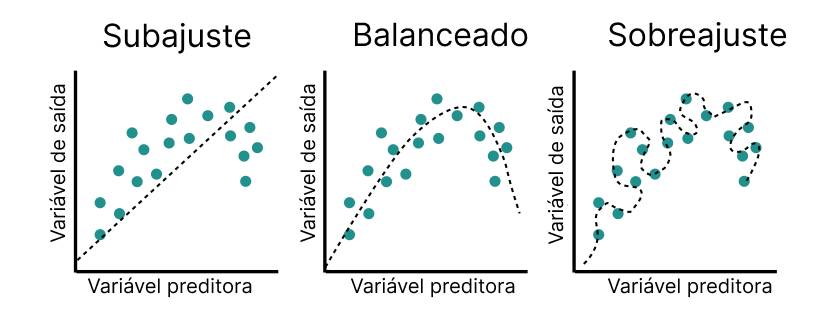
\includegraphics[width=15cm]{figures/fittings.png} % leia abaixo
	\legend{Fonte: \citeonline{educative2022overfitting}}
	\label{fig:arquitetura_cnn}
\end{figure}

\subsection{Aprendizado profundo}

O aprendizado profundo é uma área do aprendizado de máquina caracterizada por utilizar dados brutos como entrada e descobrir as representações necessárias para permitir o mapeamento adequado e assim tornando as soluções mais simples \apud{marti2017aprendizado}{lecun2015deep}.

Segundo \space\citeonline{lecun2015deep}, o aprendizado profundo são métodos de representação de aprendizado com vários níveis, obtidos por meio da decomposição de módulos simples e lineares, que transformam a representação de um nível em uma representação mais alta e abstrata. Por exemplo a representação de uma imagem é transformada em informações que identificam objetos.

Dividindo um problema complexo em problemas menores torna os métodos especializados, viabilizando tarefas mais complexas, depois essas tarefas que foram dividias são recombinadas e é gerado uma solução do problema \space\cite{marti2017aprendizado}.

Utilizando o exemplo anterior, reconhecimento de imagem, cada um desses métodos especializados seria responsável por reconhecer uma parte da imagem, como bordas, objetos, tamanho, etc. E após a junção desses métodos é feito a predição da imagem \space\cite{marti2017aprendizado}.

A principal diferença entre uma rede neural convencional e uma rede neural profunda é a quantidade de camadas, uma rede neural profunda possui várias camadas de processamento \apud{marti2017aprendizado}{haykin1999neural}.

\begin{figure}[ht]
	\centering
	\caption{Comparação de uma rede neural convencional com uma rede neural profunda.}
	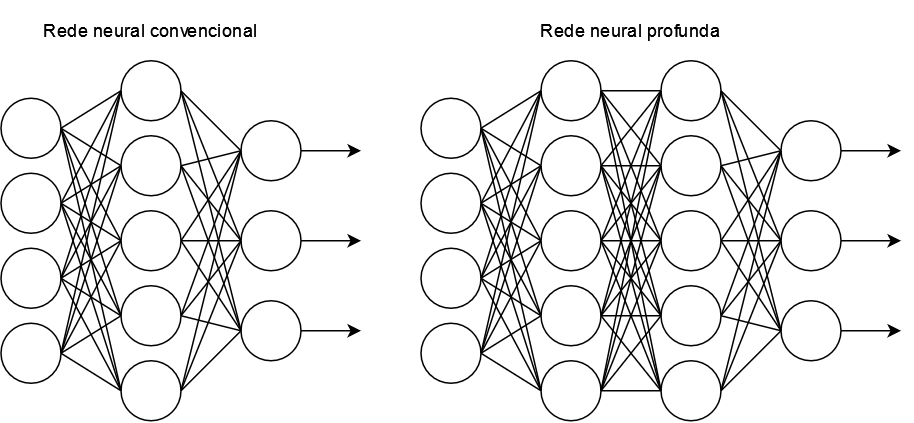
\includegraphics[width=0.8\textwidth]{figures/redes_neurais.png}
	\legend{Fonte: Criação própria}
	\label{fig:redes_neurais}
\end{figure}


\subsubsubsection{Redes neurais convolucionais}

Uma rede neural convolucional é análoga à rede neural artificial, i.e., feita de neurônios que otimizam o aprendizado através dele mesmo. A principal diferença é que a rede neural convolucional é amplamente utilizada em soluções que detectam padrões em imagens, logo existem funcionalidades específicas da própria arquitetura para essa tarefa \cite{oshea2015introduction}. 

Uma arquitetura básica de uma rede neural convolucional tem as seguintes camadas: convolucional, agrupamento e totalmente conectada. Ilustrada na \cref{fig:arquitetura_cnn} \cite{dp_overview}.

\begin{figure}[ht]
	\caption{Camadas principais de uma rede neural convolucional}
	\centering % para centralizarmos a figura
	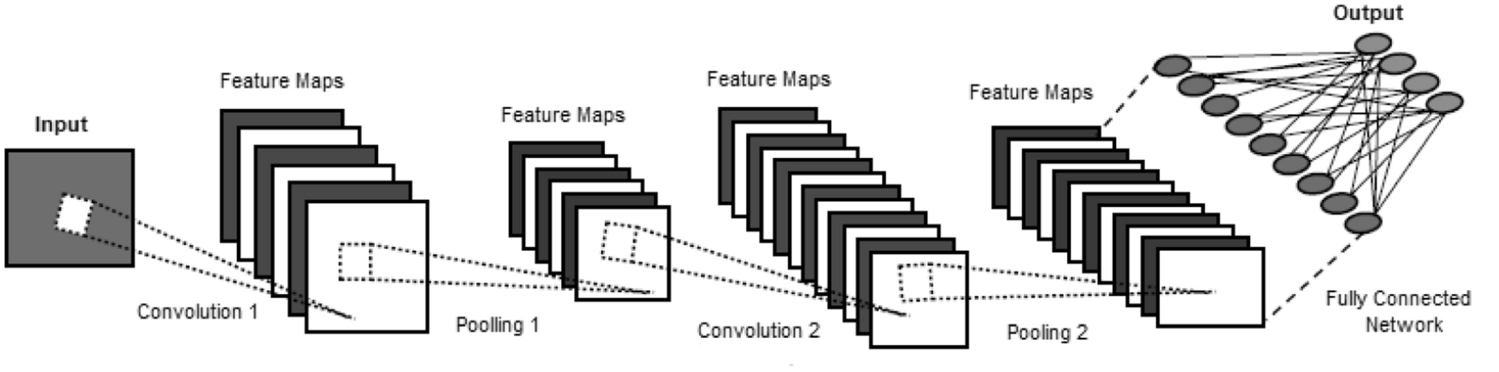
\includegraphics[width=15cm]{figures/arquitetura_cnn.png} % leia abaixo
	\legend{Fonte: \citeonline{dp_overview}}
	\label{fig:arquitetura_cnn}
\end{figure}

\subsubsubsection*{Camada convolucional}

Segundo \citeonline{computation11030052} camada convolucional é essencial para esse tipo de arquitetura e usa um filtro — ou kernel — para aplicar na imagem e direcionar para o próximo neurônio. Esse filtro é uma matriz de números que terá uma operação aplicada em todos os píxeis da imagem — que também é representado por matriz(es) — as informações cruciais para esse filtro são: tamanho, largura e pesos. Isto é utilizado para extrair características com uma base matemática, criando uma relação direta entre um píxel e os píxeis ao redor. Os pesos começam de forma pseudoaleatórias e são ajustados no decorrer do aprendizado. O resultado dessa camada é chamado de mapa de características. O tamanho da saída será baseado na fórmula abaixo sendo os tamanhos I da imagem, F do filtro e a S da saída \cite{computation11030052}.

\begin{gather}
    \mathbf{I}x - \mathbf{F}x + 1 = \mathbf{S}x \notag \\
    \mathbf{I}y - \mathbf{F}y + 1 = \mathbf{S}y
\end{gather}

    
A seguir um exemplo dos passos para construir a matriz resultante baseado em \citeonline{Alzubaidi2021}.

\clearpage

$$
\hspace{0.4cm}
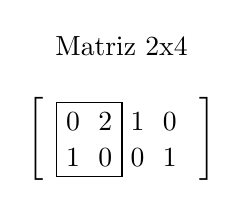
\begin{tikzpicture}[baseline=(M.center)]
 \matrix (M) [matrix of math nodes,left delimiter={[},right delimiter={]}] {
 0 & 2 & 1 & 0 \\
 1 & 0 & 0 & 1 \\
 };
 \draw (M-1-1.north west) rectangle (M-2-2.south east);
 \node[above=10pt of M.north] {Matriz 2x4};
\end{tikzpicture}
\hspace{0.8cm}\bigotimes\hspace{0.8cm}
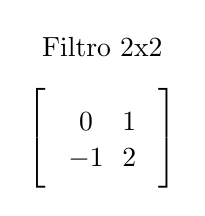
\begin{tikzpicture}[baseline=(M.center)]
 \matrix (M) [matrix of math nodes,left delimiter={[},right delimiter={]}] {
  0 & 1 \\
 -1 & 2 \\
 };
 \node[above=10pt of M.north] {Filtro 2x2};
\end{tikzpicture}
\hspace{0.8cm}=\hspace{0.8cm}
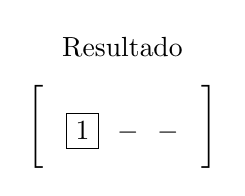
\begin{tikzpicture}[baseline=(M.center)]
 \matrix (M) [matrix of math nodes,left delimiter={[},right delimiter={]}] {
    \boxed{1} & - & - \\
 };
 \node[above=10pt of M.north] {Resultado};
\end{tikzpicture}
$$

$$
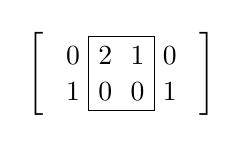
\begin{tikzpicture}[baseline=(M.center)]
 \matrix (M) [matrix of math nodes,left delimiter={[},right delimiter={]}] {
    0 & 2 & 1 & 0 \\
    1 & 0 & 0 & 1 \\
 };
 \draw (M-1-2.north west) rectangle (M-2-3.south east);
\end{tikzpicture}
\hspace{0.8cm}\bigotimes\hspace{0.8cm}
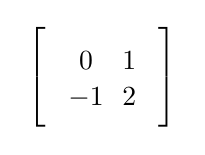
\begin{tikzpicture}[baseline=(M.center)]
 \matrix (M) [matrix of math nodes,left delimiter={[},right delimiter={]}] {
  0 & 1 \\
  -1 & 2 \\
 };
\end{tikzpicture}
\hspace{0.8cm}=\hspace{0.8cm}
\begin{bmatrix}
 1 & \boxed{1} & - \\
 \end{bmatrix}
$$

$$
\hspace{0.2cm}
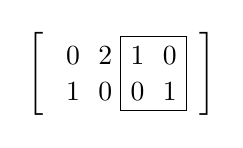
\begin{tikzpicture}[baseline=(M.center)]
 \matrix (M) [matrix of math nodes,left delimiter={[},right delimiter={]}] {
    0 & 2 & 1 & 0 \\
    1 & 0 & 0 & 1 \\
 };
 \draw (M-1-3.north west) rectangle (M-2-4.south east);
\end{tikzpicture}
\hspace{1cm}\bigotimes\hspace{0.9cm}
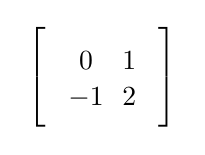
\begin{tikzpicture}[baseline=(M.center)]
 \matrix (M) [matrix of math nodes,left delimiter={[},right delimiter={]}] {
  0 & 1 \\
  -1 & 2 \\
 };
\end{tikzpicture}
\hspace{0.8cm}=\hspace{0.8cm}
\begin{bmatrix}
 1 & 1 &  \boxed{2} \\
 \end{bmatrix}
$$

\subsubsubsection*{Tamanho do passo e preenchimento}

O tamanho do passo — ou stride — serve para especificar a distância de pixels entre os passos da camada.  No exemplo acima esse parâmetro é definido como 1, por isso a matriz selecionada pula 1 pixel para direita entre os passos. Esse valor altera o tamanho da matriz resultante \cite{dp_overview}.

O preenchimento — ou padding — é uma técnica utilizada para manter o mesmo tamanho da entrada, adicionando bordas com zeros antes das operações da camada para ter como saída uma matriz da mesma dimensão da matriz original. Isso é usado devido a desvantagem em perder os detalhes nas bordas das imagens no processamento de uma camada \cite{dp_overview}.

\subsubsubsection*{Camada de agrupamento}

A camada de agrupamento — ou pooling — tem como tarefa primordial uma técnica para reduzir o tamanho do mapa de características, porém preservando os padrões mais relevantes. Dentre os recursos essenciais dessa camada estão o tamanho do agrupamento e a operação que será realizada. O maior problema dessa camada é pelo fato dela apenas identificar onde essas características estão e não se tem ou não, \emph{i.e.}, dependendo de qual operação e a quantidade de camadas pode não ser possível guardar as principais características de forma integra causando uma redução no desempenho final da predição \cite{dp_overview}.

Existem vários tipos de agrupamento, os mais utilizados são: agrupamento máximo, agrupamento médio e agrupamento global médio que estão explicados abaixo em exemplos baseados em \citeonline{Alzubaidi2021}.

\subsubsubsection*{Agrupamento máximo}

É definido o resultado com base no máximo encontrado pelo tamanho do agrupamento, exemplo a seguir usando um mapa de características com tamanho 4x4 e agrupamento de tamanho 2x2.

$$
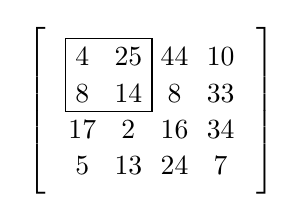
\begin{tikzpicture}[baseline=-0.5ex]
    \matrix (M) [matrix of math nodes,left delimiter={[},right delimiter={]}] {
        4 & 25 & 44 & 10\\
        8 & 14 & 8 & 33 \\
        17 & 2 & 16 & 34 \\
        5 & 13 & 24 & 7 \\
    };
    \draw (M-1-1.north west) rectangle (M-2-2.south east);
\end{tikzpicture}
= 
\begin{bmatrix}
	\boxed{25} & 44 \\
	17 & 34 \\
   \end{bmatrix}
$$

\subsubsubsection*{Agrupamento médio}

É definido o resultado com base na média encontrada pelo tamanho do agrupamento, exemplo a seguir usando um mapa de características com tamanho 4x4 e agrupamento de tamanho 2x2.

$$
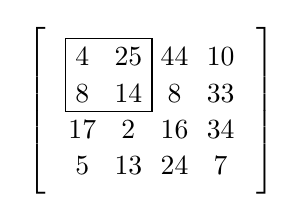
\begin{tikzpicture}[baseline=-0.5ex]
    \matrix (M) [matrix of math nodes,left delimiter={[},right delimiter={]}] {
        4 & 25 & 44 & 10\\
        8 & 14 & 8 & 33 \\
        17 & 2 & 16 & 34 \\
        5 & 13 & 24 & 7 \\
    };
    \draw (M-1-1.north west) rectangle (M-2-2.south east);
\end{tikzpicture}
= 
\begin{bmatrix}
	\boxed{12} & 23 \\
	9 & 20 \\
   \end{bmatrix}
$$

\subsubsubsection*{Agrupamento global médio}

É definido o resultado com base na média geral do mapa o que sempre tem como saída uma matrix 1x1, exemplo a seguir usando um mapa de características com tamanho 4x4.

$$
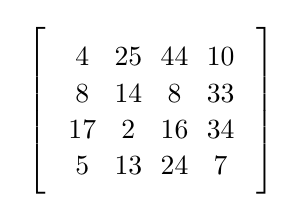
\begin{tikzpicture}[baseline=-0.5ex]
    \matrix (M) [matrix of math nodes,left delimiter={[},right delimiter={]}] {
        4 & 25 & 44 & 10\\
        8 & 14 & 8 & 33 \\
        17 & 2 & 16 & 34 \\
        5 & 13 & 24 & 7 \\
    };
\end{tikzpicture}
= 
\begin{bmatrix}
	16
   \end{bmatrix}
$$

\subsubsubsection*{Camada totalmente conectada}

A camada totalmente conectada geralmente é utilizada no final da arquitetura e cria a partir de cada neurônio uma ligação direta para cada etiqueta final. Isso torna essa camada extremamente pesada computacionalmente. O número de neurônios dessa camada é equivalente ao número de classes propostas. Além disso é quando chega nessa camada que a função de perda é calculada e se inicia a retropropagação \cite{Alzubaidi2021, computation11030052}.

\subsubsubsection*{Aperfeiçoamento}

Segundo \citeonline{Alzubaidi2021, computation11030052} existem algumas técnicas para aperfeiçoar os resultados do modelo, sendo elas:

\begin{itemize}
    \item Dropout: Muito utilizada para evitar sobreajuste pois está técnica irá desligar um neurônio aleatoriamente colocando a saída dele como zero no processo de treinamento e portanto forçara o modelo a aprender a identificar características diferentes em outros neurônios possibilitando a generalização do modelo.
    \item Aumentar o tamanho do conjunto de dados: caso não seja possível criar ou encontrar um maior existem técnicas para aumentar artificialmente acrescentando pequenas mudanças nas imagens existentes, algumas são rotacionar, recortar e inverter horizontalmente ou verticalmente.
    \item Normalização em lote: normaliza as saídas para treinar a rede mais rápido
    \item Aumentar o tempo de treinamento
    \item Aumentar a profundidade ou largura da arquitetura
    \item Ajustar os hiperparâmetros
\end{itemize}
    

\subsection{Segmentação}



\subsubsubsection*{EfficientPS}
\label{sec:EfficientPS}

EfficientPS é uma solução para a segmentação panóptica proposta no artigo \citeonline{mohan2020efficientps}, o trabalho apresenta uma arquitetura que se inicia com um backbone — parte para identificar características — usando uma Rede de Pirâmide de Características(RPC)\footnote{Estrutura de pirâmide para extrair características em várias escalas de uma imagem \space\cite{piramide}} de 2 caminhos seguido de dois cabeçotes paralelos um para uma arquitetura de segmentação semântica que é autoria deles e outra de instância com modificações baseadas na topologia Mask R-CNN e finalmente a saída dos dois cabeçotes são combinadas no módulo de fusão panóptica para gerar a saída final com a imagem de segmentação panóptica, esta arquitetura é ilustrada na \cref{fig:arqEP}.

\begin{figure}[ht]
	\caption{Arquitetura geral do EfficientPS}
	\centering % para centralizarmos a figura
	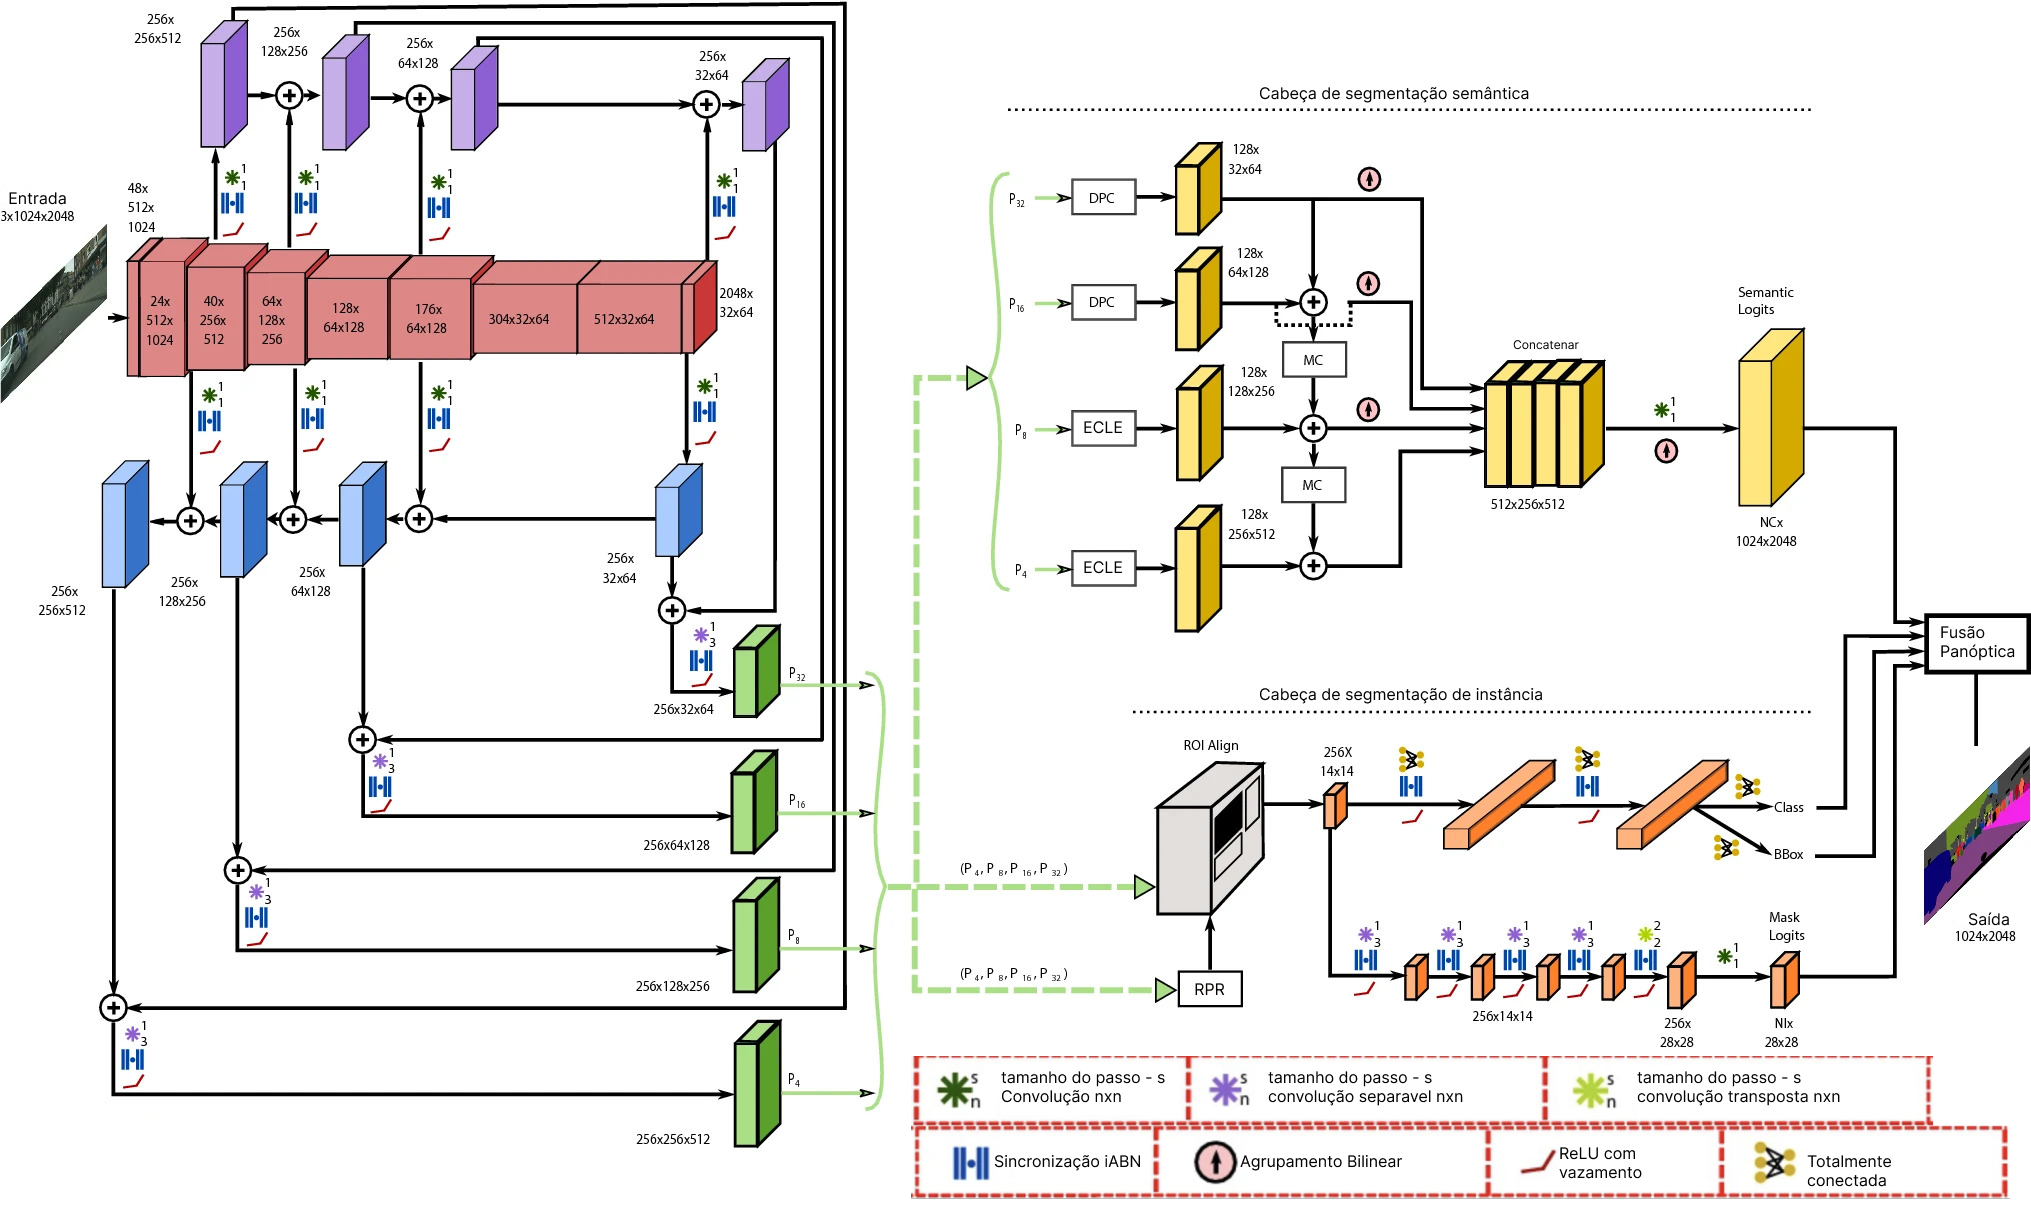
\includegraphics[width=15cm]{figures/arqEP.png} % leia abaixo
	\legend{Fonte: \citeonline{mohan2020efficientps}}
	\label{fig:arqEP}
\end{figure}

\subsubsubsection*{Backbone da rede}

A espinha dorsal — ou backbone — se consiste em uma codificação combinado a uma bifurcação paralela usando RPC. O codificador é essencial para arquiteturas de segmentação e para melhorar a capacidade de representação é necessário aumentar o número de parâmetros e a complexidade, porém nesse artigo os autores chegaram numa solução balanceada nesse quesito. O codificador contém nove blocos (em vermelho), mostrado na \cref{fig:arqEP} e a 2º, 3º, 5º e 9º saídas — da esquerda para diretira — correspondem aos fatores de redução de amostragem x4,x8,x16 e x32 respectivamente. Essas saídas vão conectar com a bifurcação paralela que são de sentidos opostos para gerar mais detecções de características. Após isso será feita uma combinação entre camadas de mesma dimensão utilizando camadas de convolução separável em profundidade — divide em etapa espacial e de canal, aplicada a cada canal e cada pixel de saída respectivamente — resultando nas saídas $ P_4 + P_8 + P_{16} + P_{32} $\cite{mohan2020efficientps, redes-neurais-convolucionais-separaveis-em-profundidade}.

\subsubsubsection*{Cabeçote de Segmentação Semântica}

O cabeçote de segmentação semântica é autoria dos autores e é dividido em três módulos sendo eles: Extrator de Características em Larga Escala (ECLE) — ou Large Scale Feature Extractor (LSFE) — para capturar recursos finos em larga escala de forma eficiente, módulo DPC deve ser capaz de capturar contexto de longo alcance, porém em pequena escala e o módulo MC deve ser capaz de mitigar a incompatibilidade entre recursos de grande e pequena escala nas camadas de agregação \space\cite{mohan2020efficientps}.

As quatro entradas do cabeçote $ P_4 + P_8 + P_{16} + P_{32} $ são separadas, sendo $ P_{16} + P_{32} $ — pequena escala — alimentam dois módulos DPC paralelos e $ P_4 + P_8 $ — larga escala — alimentam dois módulos ECLE paralelos \space\cite{mohan2020efficientps}.

\subsubsubsection*{Cabeçote de segmentação de instância}

Este cabeçote é derivada da arquitetura Mask R-CNN e as modificações foram três, sendo: trocar a convolução padrão por convolução separável em profundidade — para reduzir o número de parâmetros consumidos pela rede —, camada de normalização em lote foi substituída por iABN Sync\footnote{normalização em lotes entre cores de GPU para aumentar o desempenho} e a função ReLU definida em \cref{eq:relu_func} por Leaky ReLU definida em \cref{eq:relu_leaky_func} \space\cite{mohan2020efficientps,redes-neurais-convolucionais-separaveis-em-profundidade, serp-ai}.

\subsubsubsection*{Módulo de fusão panóptica}

O módulo da fusão panóptica é necessário para construir a imagem com segmentação panóptica. Nessa parte os resultados são unidos aos dois cabeçotes anteriormente explicados. Esta tarefa não é simples pois é necessário criar uma lógica para obter o melhor resultado diante das sobreposições encontradas. O módulo foi criado no intuito de ser adaptativo e usar as duas entradas de forma equivalente \space\cite{mohan2020efficientps}.

Resumindo o módulo aplica algumas técnicas para reduzir o número de instâncias baseando-se na métrica logist — valor numérico que pontua confiança — aplica algumas agregações entre os resultados dos dois cabeçotes e desenha com fundo preto as instâncias com melhor classificação de confiança, logo depois preenche com a parte de stuff — classes semânticas sem importância — da entrada semântica \space\cite{mohan2020efficientps}.

\section{Geração procedural de conteúdo}

Segundo \space\citeonline{yannakakis2018artificial}, em poucas palavras, a geração procedural de conteúdo constituí métodos e automações utilizados para gerar conteúdos em jogos. A geração procedural de conteúdo também é uma parte importante da inteligência artificial de um jogo e já vem sendo utilizada desde 1980.
Essa técnica pode ser utilizada para gerar níveis, mapas, textura, regras de jogo, historia, entre outras coisas.

É difícil dizer qual algoritmo foi utilizado para geração de conteúdo dos jogos modernos e os códigos fontes não são facilmente acessíveis. Já nos jogos antigos os códigos fontes e as estratégias utilizadas são acessíveis e muito bem documentadas na internet. São geralmente utilizados algoritmos de geração aleatória que podem ser classificados como sendo de força bruta, e são usados para criar estruturas ou mapas dependendo do tipo de jogo \space\cite{dormans2010adventures}.


\subsection{Diagrama de Voronoi}

Segundo \citeonline{rodrigues_diagrama_2019} diagrama de Voronoi é o particionamento do espaço onde cada região é associada a um ponto do conjunto.

O diagrama de Voronoi é gerado a partir das distancias euclidianas entre os vizinhos de um conjunto de pontos do plano\space
\cite{diagrama_de_voronoi:_uma_exploracao_nas_distancias_euclidiana_e_do_taxi}. Esse diagrama possui uma gama de utilizações, por exemplo, estudar epidemias, encontrar o 
ponto mais próximo, calcular a precipitação de uma área, estudar os padrões de crescimento das florestas, etc,\space\cite{poligonos_de_thiessen_ou_voronoi}. 

Seja um conjunto de índices $I_n = \{1, 2, 3, ..., n\}$ e $A = \{p_1, p_2, ..., p_n\} \subset \mathbb{R}^2$ um conjunto de pontos onde $2 \leq n < \infty$, definimos como região de Voronoi o conjunto de pontos associado a $p_i$, onde d é a distancia euclidiana

\begin{equation}
	V(p_i) = \{p|d(p_i,p) \leq d(p_i,p);i \neq j, i, j \in I_n\},
\end{equation}


temos o conjunto formado por essas regiões sendo $V(A) = {V(1), V(2), V(3), ..., V(n)}$ \cite{rodrigues_diagrama_2019}.

Na figura \cref{fig:diagrama_voronoi} podemos ver a relação do conjuntos de pontos com o diagrama de Voronoi.

\begin{figure}[H]
	\centering
	\caption{Diagrama de Voronoi.}
	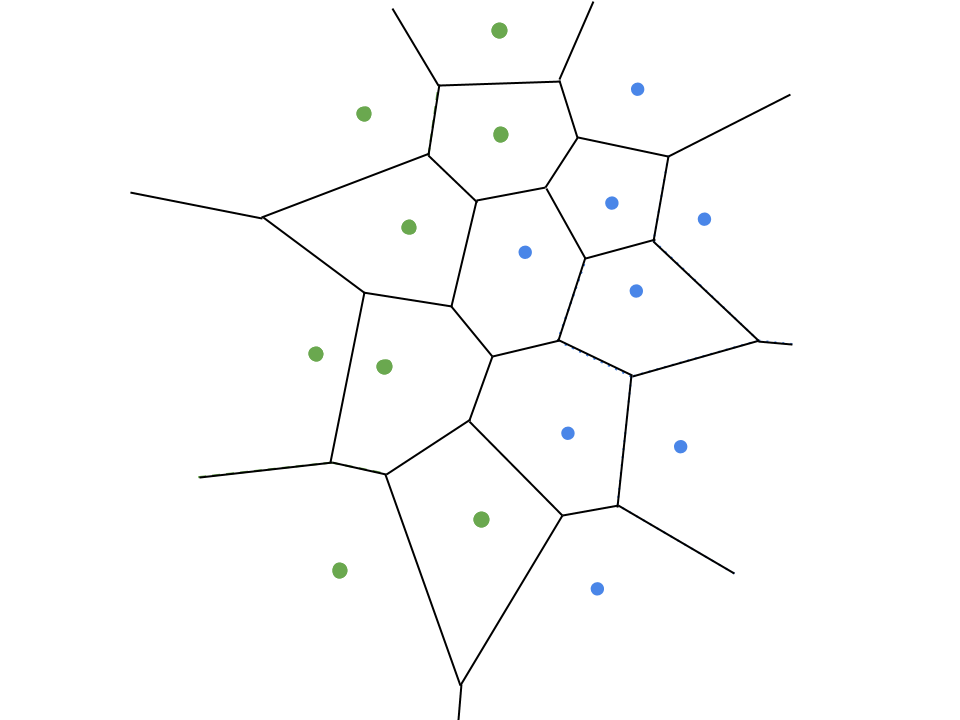
\includegraphics[width=0.8\textwidth]{figures/diagrama_de_voronoi.png}
	\legend{Fonte: \citeonline{thomazthz_diagrama_2014}}
	\label{fig:diagrama_voronoi}
\end{figure}


\subsection{Geração de biomas no diagrama de Voronoi}

Biomas são regiões ecológicas que possuem uma fauna e flora com atributos estruturais semelhantes \cite{maestrovirtuale}. Segundo \citeonline{amitp2010} o primeiro passo é gerar o litoral, essas serão as bordas que irão dizer o que é água e o que é solo. Existem algumas formas de gerar o formato da ilha:

\begin{itemize}
    \item Radial: gera ilhas circulares através de ondas senoidais.
    \item Perlin: utiliza o Perlin Noise para controlar a forma da ilha.
    \item Quadrado: preenche o mapa inteiro com solo.
\end{itemize}

É possível utilizar qualquer formato para gerar as ilhas \cite{amitp2010}, neste trabalho será utilizado o resultado da segmentação de imagem para gerar a ilha.

\begin{figure}[H]
	\caption{Diagrama de Voronoi separado em solo e mar}
	\centering % para centralizarmos a figura
	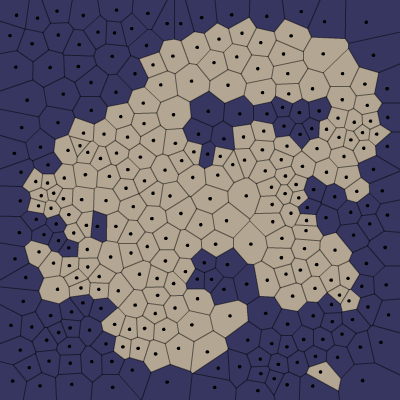
\includegraphics[width=0.7\textwidth]{figures/voronoi-land-water.png} % leia abaixo
	\legend{Fonte: \citeonline{amitp2010}}
	\label{fig:voronoi-land-water}
\end{figure}

O proximo passo é calcular a elevação do terro. A elevação será calculada através da distancia de um polígono indicado como solo até o litoral, a elevação é definida pelos cantos dos polígonos \cite{amitp2010}. 

\begin{figure}[H]
	\caption{Diagrama de Voronoi separado em solo e mar com os cantos dos polígonos indicando a direção para o litoral}
	\centering
	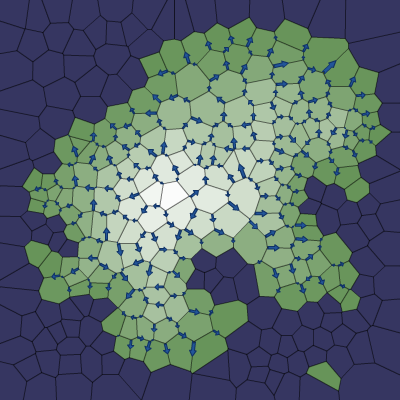
\includegraphics[width=0.7\textwidth]{figures/downslopes.png}
	\legend{Fonte: \citeonline{amitp2010}}
	\label{fig:downslopes}
\end{figure}

Com a elevação é possível gerar os biomas, um exemplo seria elevações altas significa que é uma montanha, logo ela deve possui neve. Adicionando mais uma camada, além da elevação, como a de umidade, podemos gerar uma variedade maior de biomas. A umidade é calculada de quão longe o polígino está de um corpo d'água.

\subsection*{Diagrama de Whittaker}

O diagrama de Whittaker é uma forma de dividir os terrenos gerados a partir da técnica de geração procedural, esse diagrama inclui valores de temperatura e umidade para separar os biomas \cite{wikidotwhittakerdiagram}.

\begin{figure}[H]
	\caption{Diagrama de Whittaker}
	\centering
	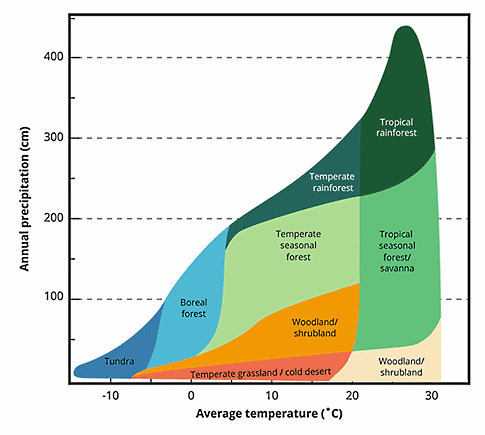
\includegraphics[width=0.6\textwidth]{figures/diagrama-whittaker.png}
	\legend{Fonte: \citeonline{mendes2019}}
	\label{fig:diagrama-whittaker}
\end{figure}

Usando a elevação como representante da temperatura de um bioma é possível utilizar o diagrama de Whittaker, fazendo alterações nesse diagrama é possível adicionar ou remover biomas \cite{amitp2010}. Com essa nova camada possibilita a adição de rios ao mapa e assim obtendo o resultado apresentado na figura \ref{fig:biomes}.

\begin{figure}[H]
	\caption{Resultado final da geração do mapa}
	\centering
	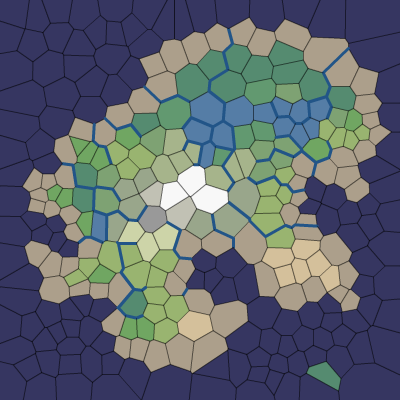
\includegraphics[width=0.5\textwidth]{figures/biomes.png}
	\legend{Fonte: \citeonline{amitp2010}}
	\label{fig:biomes}
\end{figure}




\section{Trabalhos relacionados}

Esta seção destina-se a análise e discussão da metodologia e dos resultados prospostos por \citeonline{geracao_procedural_jogos_2d,kirillov2019panoptic}. 

\subsection*{Geração Procedural de Mapas para Jogos 2D}

No trabalho \citeonline{geracao_procedural_jogos_2d}, é apresentado uma solução simples para criar mapas de cavernas, calabouços e ilhas para jogos 2D. O algoritmo foi dividido em três partes sendo elas: geração recursiva de terrenos, validação de tamanho e correção da coesão. Os autores concluíram que não existe literatura sobre geração procedural de salas diversas e corredores distintos como o algoritmo proposto. Sugerem duas possibilidades para trabalhos futuros sendo elas: usar algoritmos genéticos para mensurar a qualidade dos mapas gerados e promover pela seleção natural e a outra possibilidade é mesclar o algoritmo proposto com técnicas de geração de salas interligadas por corredores, de forma a possibilitar a criação de mapas com algumas salas pré-definidas inseridas em um mapa aberto contínuo.

\subsection*{Panoptic Segmentation}

No trabalho \citeonline{kirillov2019panoptic} é definido a ideia geral de segmentação panóptica além de definir conceitos importantes como coisas e objetos e a métrica unificada para medir o desempenho de modelos dessa área. Também é feito alguns testes comparando resultados humanos com um modelo simples proposto com eles combinando PSPNet e Mask R-CNN usando a métrica de qualidade panóptica definida por eles. Os resultados mostraram a superioridade humana na segmentação panóptica em três conjuntos de dados diferentes, sendo eles: Cityscapes, ADE20k e Vistas, as métricas usadas foram qualidade panóptica, qualidade semântica, qualidade de reconhecimento, qualidade panóptica
 de coisas e qualidade panóptica de objetos. O melhor resultado para a máquina em comparação com o humano foi no conjunto de dados Cityscapes avaliando a qualidade semântica, sendo 84,1 para o humano e 80,9 para máquina. O pior resultado para a máquina em relação ao humano foi no conjunto de dados ADE20k na qualidade panóptica de coisas, sendo 71,0 para os humanos e 24,5 para a máquina.

 \subsection*{}

\chapter{Desenvolvimento}

\section{Proposta}

Este trabalho tem como proposta a utilização de um modelo de inteligência artificial para segmentação panóptica que irá classificar os pixeis na imagem e permitir que os usuários gerem mapas procedurais a partir da seleção de um dos segmentos da imagem.

Utilizando o modelo EfficientPS é possível fazer a segmentação panóptica, segue exemplos nas \crefrange{fig:segmantations_1}{fig:segmantations_2}. O modelo citado está disponível no GitHub dos próprios autores \citeonline{mohan2020efficientps}
% e será treinado com a combinação de pelo menos dois conjuntos de dados citados anteriormente.
 No resultado apenas será identificado os pixeis de classes contidas nos conjuntos de dados escolhidos, portanto é possível que em uma imagem não seja identificado nada:

\begin{figure}[!ht]
	\centering
    \caption{Imagem de entrada para rede neural.}
	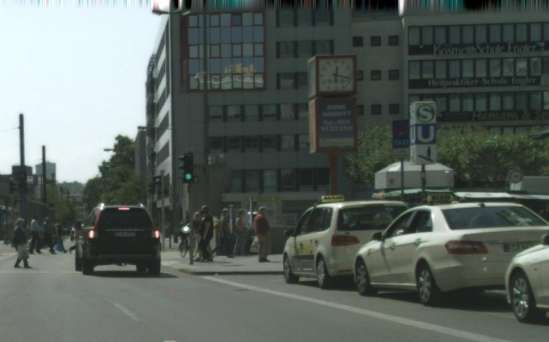
\includegraphics[width=0.6\textwidth]{figures/segmantations_1.png}
    \legend{Fonte: \citeonline{kirillov2019panoptic}}
	\label{fig:segmantations_1}
\end{figure}

\begin{figure}[!ht]
	\centering
    \caption{Imagem saída de um modelo de segmentação panóptica de segmentação panóptica.}
	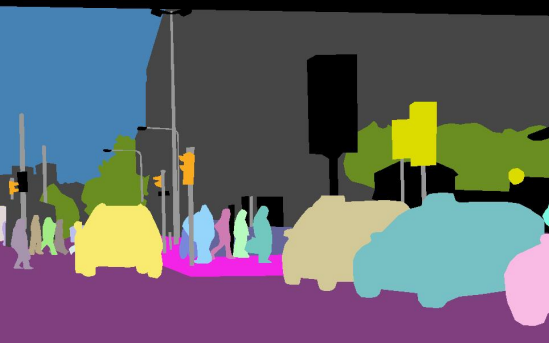
\includegraphics[width=0.6\textwidth]{figures/segmantations_2.png}
    \legend{Fonte: \citeonline{kirillov2019panoptic}}
	\label{fig:segmantations_2}
\end{figure}

Após a segmentação da imagem o usuário poderá selecionar qual parte da imagem será utilizada para gerar a ilha.

Feito a seleção será gerado um diagrama de Voronoi que funcionará como um filtro em cima dessa imagem, assim gerando a ilha e os biomas.

\begin{figure}[!ht]
	\centering
    \caption{Ilha gerada a partir da segmentação panóptica e aplicando um filtro com o diagrama de Voronoi, azul representa oceano, verde floresta, cinza montanhas.}
	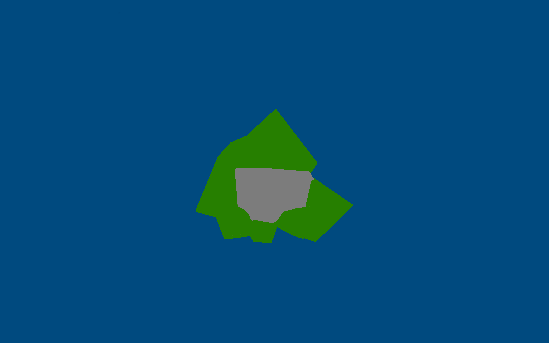
\includegraphics[width=0.6\textwidth]{figures/segmantations_pnl.png}
    \legend{Fonte: Criação própria}
	\label{fig:segmantations_pnl}
\end{figure}



\section{Cronograma}

O processo de desenvolvimento será separado em 3 tópicos principais, inteligência artificial, diagrama de Voronoi e interface de usuário. O desenvolvimento de cada tópico do software será feito em paralelo, pois os tópicos não possuem acoplamento.

\subsection*{inteligência Artificial}

Será necessário decidir quais conjuntos de dados utilizar, o modelo está pronto e disponível no GitHb \cite{mohan2020efficientps} portanto será necessário treinar o modelo e avalia-lo com base na métrica PQ \cref{eq:pq_metric}.

As especificações do modelo proposto são: Linux, Python 3.7, PyTorch 1.7, CUDA 10.2, GCC 7 ou 8 além dos pacotes inseridos no arquivo requirements.txt.

O tempo estimado para o desenvolvimento é de 1 a 2 meses, a maior parte será para treinar e validar o resultado.

\subsection*{Diagrama de Voronoi}

Para o desenvolver código do diagrama de Voronoi será preciso primeiro gerar os pontos e desses pontos as áreas, fazer o algoritmo entender se a área tocou no segmento de imagem, caso tenha tocado armazenar para um processamento posterior que irá especificar qual bioma aquela áreas será, para fazer os teste será necessário uma imagem com um polígono.

O tempo estimado para o desenvolvimento é de 1 mes.

\subsection*{Interface de Usuário}

A interface de usuário terá 5 telas principais, inicio, processamento da segmentação, seleção, processamento de seleção, resultado. 

As telas terão o seguinte fluxo:

\begin{figure}[H]
	\centering
    \caption{Tela de início, botões de carregar imagem e carregar projeto, menu de contexto arquivos com 3 botões, carregar imagem, carregar projeto e salvar.}
	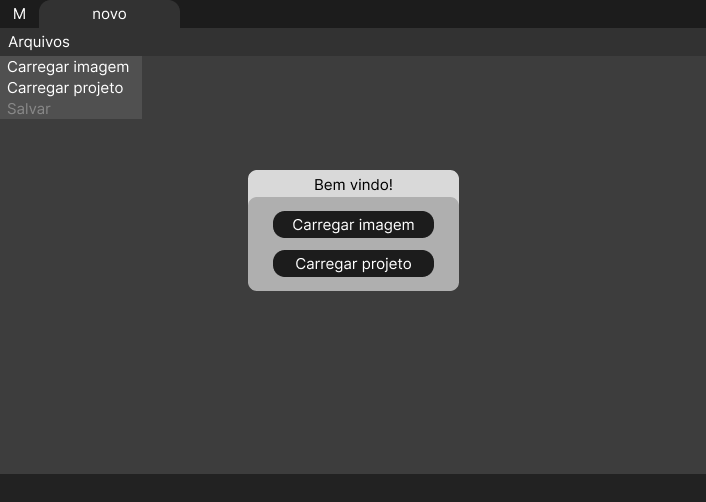
\includegraphics[width=0.6\textwidth]{figures/tela_novo.png}
    \legend{Fonte: Criação própria}
	\label{fig:tela_novo}
\end{figure}


\begin{figure}[H]
	\centering
    \caption{Tela de processamento da segmentação}
	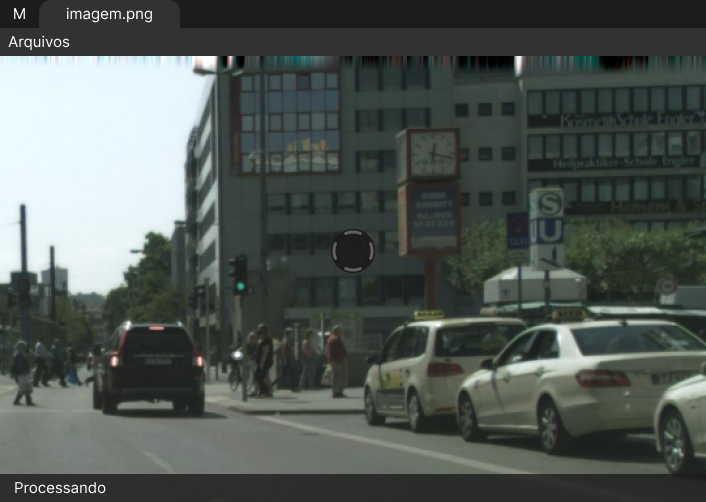
\includegraphics[width=0.6\textwidth]{figures/tela_processando_1.png}
    \legend{Fonte: Criação própria}
	\label{fig:tela_processando_1}
\end{figure}


\begin{figure}[H]
	\centering
    \caption{Tela de seleção de segmentação da imagem.}
	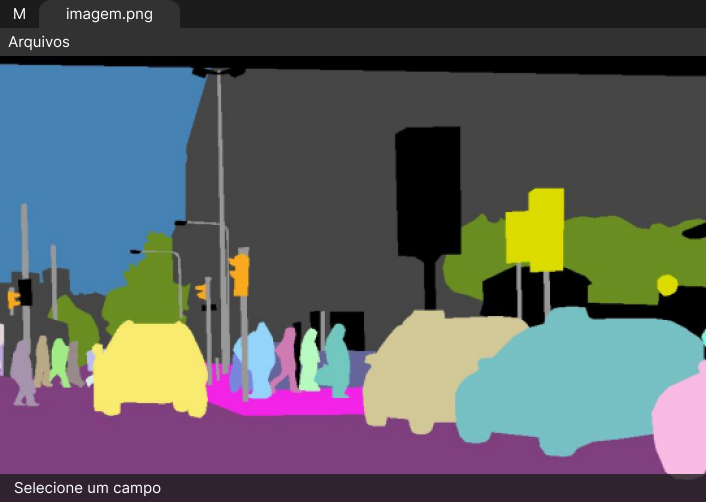
\includegraphics[width=0.6\textwidth]{figures/tela_carregado.png}
    \legend{Fonte: Criação própria}
	\label{fig:tela_carregado}
\end{figure}


\begin{figure}[H]
	\centering
    \caption{Tela de processamento para geração do mapa com a seleção do segmento.}
	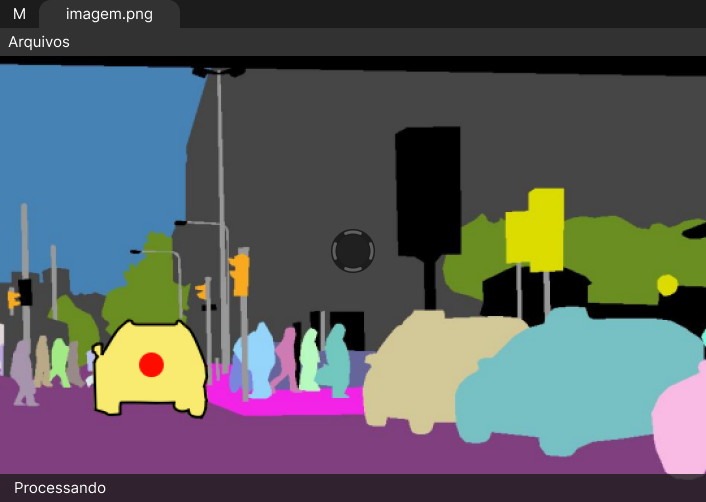
\includegraphics[width=0.6\textwidth]{figures/tela_processando_2.png}
    \legend{Fonte: Criação própria}
	\label{fig:tela_processando_2}
\end{figure}


\begin{figure}[H]
	\centering
    \caption{Tela de resultado com o mapa gerado após processamento.}
	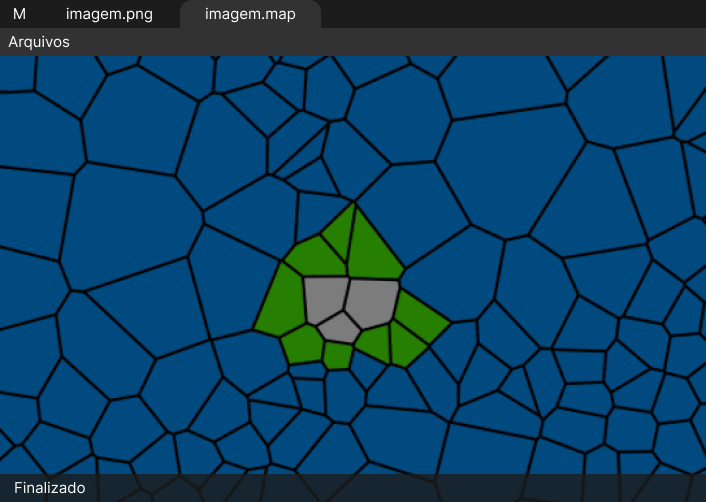
\includegraphics[width=0.6\textwidth]{figures/tela_mapa.png}
    \legend{Fonte: Criação própria}
	\label{fig:tela_mapa}
\end{figure}

Após isso a interface permitirá o usuário salvar o projeto bem como exportar o resultado.

O tempo de desenvolvimento será em torno de 1 mês.

% ----------------------------------------------------------
% Finaliza a parte no bookmark do PDF
% para que se inicie o bookmark na raiz
% e adiciona espaço de parte no Sumário
% ----------------------------------------------------------
%\phantompart

% ---
% Conclusão (outro exemplo de capítulo sem numeração e presente no sumário)
% ---
\chapter*[Conclusão]{Conclusão}
\addcontentsline{toc}{chapter}{Conclusão}
% ---

\lipsum[31-33]

% ----------------------------------------------------------
% ELEMENTOS PÓS-TEXTUAIS
% ----------------------------------------------------------
\postextual
% ----------------------------------------------------------

% ----------------------------------------------------------
% Referências bibliográficas
% ----------------------------------------------------------
\bibliography{references}

% ----------------------------------------------------------
% Glossário
% ----------------------------------------------------------
%
% Consulte o manual da classe abntex2 para orientações sobre o glossário.
%
%\glossary

% ----------------------------------------------------------
% Apêndices
% ----------------------------------------------------------

% ---
% Inicia os apêndices
% ---
% \begin{apendicesenv}

% % Imprime uma página indicando o início dos apêndices
% \partapendices

% % ----------------------------------------------------------
% \chapter{Quisque libero justo}
% % ----------------------------------------------------------

% \lipsum[50]

% % ----------------------------------------------------------
% \chapter{Nullam elementum urna vel imperdiet sodales elit ipsum pharetra ligula
% ac pretium ante justo a nulla curabitur tristique arcu eu metus}
% % ----------------------------------------------------------
% \lipsum[55-57]

% \end{apendicesenv}
% ---


% ----------------------------------------------------------
% Anexos
% ----------------------------------------------------------

% ---
% Inicia os anexos
% ---
% \begin{anexosenv}

% % Imprime uma página indicando o início dos anexos
% \partanexos

% % ---
% \chapter{Morbi ultrices rutrum lorem.}
% % ---
% \lipsum[30]

% % ---
% \chapter{Cras non urna sed feugiat cum sociis natoque penatibus et magnis dis
% parturient montes nascetur ridiculus mus}
% % ---

% \lipsum[31]

% % ---
% \chapter{Fusce facilisis lacinia dui}
% % ---

% \lipsum[32]

% \end{anexosenv}

%---------------------------------------------------------------------
% INDICE REMISSIVO
%---------------------------------------------------------------------
%\phantompart
\printindex
%---------------------------------------------------------------------

\end{document}